\documentclass[11pt,a4paper]{article}

% ============================ packages ============================
\usepackage[utf8]{inputenc}
\usepackage[T1]{fontenc}

\usepackage[margin=1in]{geometry}
\usepackage{amsmath,amssymb,amsthm,mathtools}
\usepackage{bm}
\usepackage{graphicx}
\usepackage{booktabs}
\usepackage{array}
\usepackage{multirow}
\usepackage{caption}
\usepackage{subcaption}
\usepackage{enumitem}
\usepackage{xcolor}
\usepackage{hyperref}
\hypersetup{
    colorlinks=true,
    linkcolor=blue!50!black,
    citecolor=blue!50!black,
    urlcolor=blue!60!black,
}
\usepackage{cleveref}
\usepackage{listings}

% --------- code style ---------
\definecolor{codebg}{rgb}{0.97,0.97,0.97}
\definecolor{codekw}{rgb}{0.12,0.12,0.55}
\definecolor{codestr}{rgb}{0.55,0.10,0.10}
\definecolor{codecom}{rgb}{0.30,0.50,0.30}
\definecolor{codenum}{rgb}{0.50,0.50,0.50}

\lstdefinestyle{pystyle}{
    backgroundcolor=\color{codebg},
    basicstyle=\ttfamily\footnotesize,
    keywordstyle=\color{codekw}\bfseries,
    commentstyle=\color{codecom}\itshape,
    stringstyle=\color{codestr},
    numberstyle=\tiny\color{codenum},
    numbers=left,
    numbersep=6pt,
    breaklines=true,
    captionpos=b,
    frame=single,
    framerule=0.3pt,
    rulecolor=\color{black!30},
    tabsize=4,
    showstringspaces=false,
    language=Python,
    morekeywords={None,True,False,as,async,await,nonlocal,with,yield,self,cls},
    aboveskip=8pt,
    belowskip=8pt,
}
\lstset{style=pystyle}

% --------- shorthand macros ---------
\newcommand{\R}{\mathbb{R}}
\newcommand{\N}{\mathbb{N}}
\newcommand{\E}{\mathbb{E}}
\newcommand{\norm}[1]{\left\lVert #1 \right\rVert}
\newcommand{\abs}[1]{\left\lvert #1 \right\rvert}
\newcommand{\inner}[2]{\langle #1,\, #2\rangle}
\newcommand{\diag}{\operatorname{diag}}
\newcommand{\diagext}{\operatorname{diag_{ext}}}
\newcommand{\rank}{\operatorname{rank}}
\newcommand{\Order}{\mathcal{O}}
\newcommand{\Alin}{A_{\mathrm{lin}}}
\newcommand{\Glin}{G_{\mathrm{lin}}}
\newcommand{\GK}{G_{K}}
\newcommand{\hK}{h_{K}}
\newcommand{\Bt}{B^{\!\top}}
\newcommand{\Jt}{J^{\!\top}}
\newcommand{\Phit}{\Phi^{\!\top}}
\newcommand{\Jut}{J_{u}^{\!\top}}
\newcommand{\Atop}{A_{\mathrm{top}}}

\newtheorem{lemma}{Lemma}
\newtheorem{proposition}{Proposition}
\newtheorem{remark}{Remark}

% ============================ title ============================
\title{
  \vspace{-1.2cm}
  \textbf{Fast Dense Solvers for Spectral Physics-Informed\\
  Neural Networks via Gauss--Newton Compression}\\[3pt]
  \large A Sherman--Morrison--Woodbury and Matrix-Free LSQR Study\\[2pt]
  \large on One-Dimensional Boundary-Value Problems
}
\author{Research Report}
\date{\today}

\begin{document}

\maketitle

\begin{abstract}
We study Gauss--Newton (GN) optimisation of spectral physics-informed neural networks
(PINNs) for two boundary-value problems on $[-1,1]$ with homogeneous Dirichlet
conditions: the linear problem $-u'' = f$ and the nonlinear problem
$-u'' + u^{3} = f$. The solution is parameterised as
$u_{\theta}(x) = \Phi(x)\, c(\theta)$ where $\Phi$ is a Chebyshev basis evaluated at
Chebyshev--Gauss--Lobatto (CGL) collocation nodes and $c(\theta)\in\R^{K}$ is the
output of a small multilayer perceptron with $P$ parameters. Because
$\rank(\partial r/\partial\theta) \le K \ll P$, the GN normal equations are
rank-deficient and a Levenberg--Marquardt (LM) damping is required.
We compare three solvers of the damped normal system: (i)~a strong dense baseline
using LAPACK \texttt{lstsq} (linear) or SciPy \texttt{least\_squares} with the
analytic Jacobian (nonlinear); (ii)~a Sherman--Morrison--Woodbury (SMW) compression
that reduces the $P\times P$ system to a $K\times K$ solve; and (iii)~a matrix-free
LSQR solver that never materialises the Jacobian. On the nonlinear problem at
$N=2000$ collocation points, the SMW method is \textbf{$209\times$ faster} than
the dense baseline (786\,ms vs 164\,s) at comparable relative $L^{2}$ accuracy
($\sim\!10^{-6}$ vs $10^{-11}$); the matrix-free LSQR variant gives a $111\times$
speedup at the same $N$. Ablation studies sweeping the basis truncation $K$,
the LSQR inner-iteration count, and the network initialisation reveal that
zero-initialisation of the output layer is essential at large $N$ on the
nonlinear problem (Xavier-init fails outright at $N=1000$), and that LSQR's
matrix-free advantage does \emph{not} transfer to large $K$ on this problem
class because its required inner-iteration count grows superlinearly in $K$.
A per-LM-step cost breakdown attributes most of M1's runtime to the
$\Order((N{+}1)K^{2})$ Gram-matrix assembly at large $N$.
This report documents the full methodology, gives the derivation of both compressed
solvers, lists the complete implementation, and analyses the speed--accuracy
trade-offs.
\end{abstract}

\tableofcontents
\bigskip\hrule\bigskip

% ============================ Introduction ============================
\section{Introduction}
\label{sec:intro}

\subsection{Motivation}

Physics-informed neural networks parameterise the solution of a PDE as a
neural network and minimise the PDE residual on a collocation grid. The natural
loss is a least-squares functional, which motivates second-order optimisation:
Gauss--Newton or Levenberg--Marquardt. However, when the network has $P$
parameters and the collocation grid has $N$ points, the GN normal equations
involve $P\times P$ matrices that are prohibitively expensive to assemble and
factor at every outer iteration.

A specific structure rescues us in the spectral PINN setting. If the network
output is the coefficient vector of a fixed truncated polynomial expansion
\begin{equation}
\label{eq:param}
u_{\theta}(x) = \Phi(x)\, c(\theta), \qquad c(\theta)\in\R^{K},
\end{equation}
with $K$ fixed and much smaller than $P$, then the Jacobian of the residual with
respect to $\theta$ factors through a $K$-dimensional bottleneck:
\begin{equation}
\label{eq:Jfactor}
J = J_{u}(u)\,\Phi\, B, \qquad B := \partial c / \partial \theta \in\R^{K\times P}.
\end{equation}
Consequently $\rank(J) \le K \ll P$, and the damped normal equations
$\bigl(\Bt G_{K} B + \mu I_{P}\bigr)\Delta\theta = -\Bt h_{K}$ admit
\emph{Woodbury-type} compression to a $K\times K$ solve.

\subsection{Contributions}

\begin{enumerate}[leftmargin=*]
    \item We give a clean derivation of the SMW-compressed Gauss--Newton step
        for spectral PINNs (\Cref{sec:smw}), in a form that avoids forming
        $G_{K}^{-1}$ and avoids any inner line search by relying on adaptive LM
        damping. We exploit the structure $J_{u} = \Alin + E$ where $E$ is a
        $u$-dependent diagonal supported on the PDE rows to reduce $G_{K}$
        updates to $\Order((N+1)K)$ per iteration.
    \item We give the corresponding matrix-free LSQR formulation
        (\Cref{sec:lsqr}) with explicit forward and adjoint operators of cost
        $\Order(KP + (N+1)K)$ each, and verify adjoint consistency to round-off.
    \item We benchmark all three solvers on the linear and nonlinear BVPs
        across nine grid sizes $N\in\{40, 80, 120, 160, 250, 500, 1000,$
        $1500, 2000\}$. The empirical scaling matches the predicted $\Order(N)$ vs $\Order(N^{3})$
        cost, giving $209\times$ and $111\times$ speedup at $N=2000$ for the
        SMW and LSQR methods respectively.
    \item We document the failure mode of the dense baseline at $N=2000$ in the
        linear case (LAPACK \texttt{gelsd} returns garbage) and explain why
        the network reparameterisation is itself a regularisation.
    \item We perform three ablation studies (\Cref{sec:ablations}) that
        defend the four main hyperparameter choices and reveal a counterintuitive
        finding: M2 (LSQR) does \emph{not} overtake M1 (SMW) as $K$ grows,
        because the LSQR inner-iteration count required for LM acceptance
        scales as $cK$ with a growing prefactor $c$ rather than the textbook
        $K$. We also report a per-LM-step cost breakdown showing that the
        $\Order((N+1)K^{2})$ Gram-assembly term dominates M1's wall time at
        $N\ge 1000$.
\end{enumerate}

\subsection{Notation}

Lowercase bold-italic letters denote vectors and uppercase Roman letters denote
matrices. $\Phi\in\R^{(N+1)\times K}$ is the Chebyshev basis matrix evaluated at
the CGL nodes; $\Alin\in\R^{(N+3)\times(N+1)}$ is the discrete linear operator
augmented with two boundary-condition rows of weight $\lambda$. We use
$\diagext(v)$ for the embedding of $v\in\R^{N+1}$ as a diagonal supported on
the top $N+1$ rows of an $(N+3)\times(N+1)$ block. The Frobenius norm is
$\norm{\cdot}_{F}$ and the spectral $\ell^{2}$ norm is $\norm{\cdot}_{2}$.

% ============================ Problem ============================
\section{Problem Setup}
\label{sec:problem}

\subsection{The two BVPs}

Both problems are posed on $x\in[-1,1]$ with homogeneous Dirichlet boundary
conditions $u(\pm 1) = 0$. We use the manufactured solution
$u^{\star}(x) = \sin(\pi x)$ so that exact-solution errors can be measured.

\paragraph{Problem A (linear).}
\begin{equation}
-u''(x) = f(x), \qquad f(x) = \pi^{2}\sin(\pi x).
\label{eq:probA}
\end{equation}

\paragraph{Problem B (nonlinear).}
\begin{equation}
-u''(x) + u(x)^{3} = f(x), \qquad f(x) = \pi^{2}\sin(\pi x) + \sin^{3}(\pi x).
\label{eq:probB}
\end{equation}

\subsection{Chebyshev pseudospectral discretisation}

We collocate on the $N+1$ Chebyshev--Gauss--Lobatto (CGL) nodes,
\begin{equation}
x_{j} = \cos\!\left(\frac{j\pi}{N}\right), \qquad j=0,1,\ldots,N,
\end{equation}
and use the standard CGL differentiation matrix
$D\in\R^{(N+1)\times(N+1)}$ \cite[Eq.~6.4]{trefethen2000}. The PDE operator is
$-D^{2}$, and we encode the two boundary conditions by augmenting with weighted
identity rows:
\begin{equation}
\Alin =
\begin{bmatrix}
-D^{2} \\[2pt] \lambda\, e_{0}^{\!\top}\\[2pt] \lambda\, e_{N}^{\!\top}
\end{bmatrix}
\in\R^{(N+3)\times(N+1)}, \qquad \lambda = 10.
\label{eq:Alin}
\end{equation}
The discrete RHS is
$\tilde f = [f(x_{0}),\ldots,f(x_{N}),\, 0,\, 0]^{\top}\in\R^{N+3}$. The
nonlinear discrete residual is
\begin{equation}
F(u) = \Alin\, u + g(u) - \tilde f,
\qquad
g(u) =
\begin{cases}
[u^{3};\,0;\,0]\in\R^{N+3} & \text{(nonlinear)}\\
0 & \text{(linear)}.
\end{cases}
\end{equation}
The Jacobian of $F$ with respect to $u$ is
\begin{equation}
J_{u}(u) = \Alin + E(u), \qquad
E(u) = \diagext\!\bigl(3u^{2}\bigr).
\label{eq:Ju}
\end{equation}
Here $\diagext(v)$ denotes the $(N+3)\times(N+1)$ matrix whose top
$N+1\times N+1$ block is $\diag(v)$ and whose bottom two rows are zero;
$E\equiv 0$ in the linear case.

\subsection{Why a small Chebyshev basis suffices}

For analytic $u^{\star}$, the Chebyshev expansion converges geometrically. For
$u^{\star}(x) = \sin(\pi x)$ in particular, machine precision is reached
already at $K\approx 15$. We verify this empirically by projecting $u^{\star}$
onto $\Phi$ via least squares and reporting $\norm{\Phi\, c - u^{\star}}_{2}/\norm{u^{\star}}_{2}$:

\medskip
\begin{center}
\begin{tabular}{rl}
\toprule
$K$ & projection error \\
\midrule
$4$  & $1.7\times 10^{-2}$ \\
$8$  & $4.6\times 10^{-7}$ \\
$12$ & $1.6\times 10^{-12}$ \\
$16$ & $2.5\times 10^{-16}$ \\
$20$ & $2.5\times 10^{-16}$ \\
$30$ & $4.2\times 10^{-16}$ \\
\bottomrule
\end{tabular}
\end{center}
\medskip

\noindent This is the structural fact that makes the SMW compression effective:
\textbf{we can fix $K=20$ for every collocation grid size $N$}, so the $K\times K$
solve in the SMW method has bounded cost while $N$ grows.

\subsection{Spectral PINN parameterisation}

The numerical solution is
$u_{\theta} = \Phi\, c(\theta)\in\R^{N+1}$, where $c:\R^{P}\to\R^{K}$ is a
small multilayer perceptron fed a constant input,
\begin{equation}
c(\theta) = W_{3}\,\tanh\!\bigl(W_{2}\tanh(W_{1}\cdot 1 + b_{1}) + b_{2}\bigr) + b_{3},
\label{eq:mlp}
\end{equation}
with hidden width $H=8$ and $P\approx 200$ parameters. We zero-initialise the
output layer ($W_{3} = 0$, $b_{3} = 0$) so that the initial coefficient vector
is exactly zero and the first GN step starts from $u\equiv 0$. This is
practically important at large $N$ where the residual norm $\norm{\tilde f}_{2}$
is large and a random initialisation can give an initial residual that overflows
the LM trust region.

The Jacobian $B := \partial c/\partial\theta\in\R^{K\times P}$ is computed in
one vectorised reverse-mode call with \texttt{torch.func.jacrev}, replacing the
naive $K$-step backward loop.

% ============================ Gauss-Newton structure ============================
\section{Gauss--Newton Normal Equations and Their Structure}
\label{sec:gn}

The residual we minimise is $r(\theta) := F\bigl(\Phi c(\theta)\bigr)\in\R^{N+3}$.
By the chain rule,
\begin{equation}
J(\theta) = \frac{\partial r}{\partial \theta} = J_{u}\!\bigl(\Phi c(\theta)\bigr)\,\Phi\, B(\theta) \;\in\; \R^{(N+3)\times P}.
\label{eq:Jchain}
\end{equation}

\subsection{The key rank observation}

\begin{proposition}[Low-rank factorisation]
\label{prop:rank}
For every $\theta$, $\rank\bigl(J(\theta)\bigr) \le K$.
\end{proposition}

\begin{proof}
$J = (J_{u}\Phi)\,B$ where $J_{u}\Phi\in\R^{(N+3)\times K}$ and $B\in\R^{K\times P}$.
The rank of a product is bounded by the smaller of the inner dimensions.
\end{proof}

\noindent Since $K\ll P$, the Gauss--Newton normal equations $\Jt J\, \Delta\theta
= -\Jt r$ form a $P\times P$ system of rank at most $K$. Direct factorisation of
this $P\times P$ system is wasteful; the Levenberg--Marquardt damping reads
\begin{equation}
\bigl(\Bt \GK B + \mu I_{P}\bigr)\,\Delta\theta = -\Bt \hK,
\label{eq:damped}
\end{equation}
where we have introduced the $K$-dimensional Gram matrix and gradient
\begin{equation}
\GK := (J_{u}\Phi)^{\!\top}\!(J_{u}\Phi) \in\R^{K\times K}, \qquad
\hK := \Phit\, \Jut\, r \in\R^{K}.
\label{eq:GKhK}
\end{equation}

\subsection{Cheap incremental updates to $\GK$ in the nonlinear case}

In the linear case $J_{u} = \Alin$ is constant, so
$\GK = (\Alin\Phi)^{\!\top}(\Alin\Phi) =: \Glin$ is computed once.

In the nonlinear case, expand
$J_{u}\Phi = \Alin\Phi + E\Phi$ to obtain
\begin{equation}
\GK = \Glin
   + \Phit\,\Alin^{\!\top} E\, \Phi
   + \bigl(\Phit\,\Alin^{\!\top} E\, \Phi\bigr)^{\!\top}
   + \Phit E^{2}\Phi.
\label{eq:GKupdate}
\end{equation}
Because $E$ is diagonal with support only on the top $N+1$ rows, each cross-term
reduces to operations restricted to the top $N+1\times N+1$ block of $\Alin$.
The dominant work is one $(N+1)\times K$ matrix multiplication per cross-term,
costing $\Order((N+1)K^{2})$ in total. The right-hand side $\hK$ admits the
analogous decomposition
\begin{equation}
\hK = \Phit\Alin^{\!\top} r + \Phit\,(e \odot r_{1:N+1}),
\qquad e = 3 u^{2}.
\end{equation}

% ============================ Methods ============================
\section{Three Solvers for the Damped Normal Equations}
\label{sec:methods}

\subsection{Method 0 (M0): Dense baseline}
\label{sec:m0}

For Problem A we solve $\Alin u = \tilde f$ directly with
\texttt{numpy.linalg.lstsq} (LAPACK \texttt{gelsd}). For Problem B we run
\texttt{scipy.optimize.least\_squares} with method \texttt{'lm'} and the
\emph{analytic} Jacobian $J_{u}$ from~\eqref{eq:Ju}; this is a strong baseline
because it avoids finite-difference Jacobian evaluations. Cost per LM step is
$\Order(N^{3})$ from the dense factorisation of the $(N+3)\times(N+1)$ Jacobian.

\subsection{Method 1 (M1): Sherman--Morrison--Woodbury compression}
\label{sec:smw}

\begin{lemma}[Woodbury compression]
\label{lem:smw}
Let $\GK\in\R^{K\times K}$ be symmetric positive semidefinite, $B\in\R^{K\times P}$,
$g_{P}\in\R^{P}$, and $\mu > 0$. Define
\begin{equation}
M := \mu \GK^{-1} + B \Bt \in\R^{K\times K}.
\label{eq:Mdef}
\end{equation}
Then the unique solution $\Delta\theta\in\R^{P}$ of
$(\mu I_{P} + \Bt \GK B)\,\Delta\theta = -g_{P}$
satisfies
\begin{equation}
\Delta\theta = -\tfrac{1}{\mu}\bigl(g_{P} - \Bt y\bigr), \qquad
M y = B g_{P}.
\label{eq:smwfinal}
\end{equation}
Furthermore, the system $M y = B g_{P}$ can be rewritten without forming
$\GK^{-1}$ as
\begin{equation}
\bigl(\mu I_{K} + \GK B \Bt\bigr)\, y = \GK\, B g_{P}.
\label{eq:smwequiv}
\end{equation}
\end{lemma}

\begin{proof}
The Sherman--Morrison--Woodbury identity gives
$(\mu I_{P} + \Bt \GK B)^{-1} = \tfrac{1}{\mu}\bigl[I_{P} - \Bt M^{-1} B\bigr]$
with $M$ as in~\eqref{eq:Mdef}. Therefore
\begin{align*}
\Delta\theta
&= -\tfrac{1}{\mu}\bigl[I - \Bt M^{-1} B\bigr]\, g_{P}\\
&= -\tfrac{1}{\mu}\bigl[g_{P} - \Bt (M^{-1} B g_{P})\bigr]\\
&= -\tfrac{1}{\mu}\bigl[g_{P} - \Bt y\bigr],
\end{align*}
where $y = M^{-1} B g_{P}$ solves $M y = B g_{P}$. Left-multiplying $M$ in this
last equation by $\GK$ gives~\eqref{eq:smwequiv}.
\end{proof}

\begin{remark}
Equation~\eqref{eq:smwequiv} is the workhorse. We never compute $\GK^{-1}$, and
the matrix $\mu I_{K} + \GK B\Bt$ is small ($K\times K$) and well-conditioned for
moderate $\mu$. With $g_{P} = \Bt \hK$, the M1 step is summarised:
\begin{enumerate}
    \item Form $g_{P} = \Bt \hK$, $B g_{P}\in\R^{K}$, and $B\Bt\in\R^{K\times K}$.
    \item Build $\GK$ via the structural update~\eqref{eq:GKupdate}.
    \item Solve $\bigl(\mu I_{K} + \GK B\Bt\bigr)\, y = \GK B g_{P}$.
    \item Return $\Delta\theta = -\tfrac{1}{\mu}(g_{P} - \Bt y)$.
\end{enumerate}
Total cost per LM step is $\Order\bigl(K^{3} + K^{2}P + (N+1)K^{2}\bigr)$, which
for fixed $K$ and growing $N$ is $\Order(N)$.
\end{remark}

\subsection{Method 2 (M2): Matrix-free LSQR}
\label{sec:lsqr}

LSQR (Paige--Saunders, 1982) solves the damped least-squares problem
\begin{equation}
\min_{\Delta\theta}\;\left\Vert
\begin{bmatrix} J \\ \sqrt{\mu}\, I_{P} \end{bmatrix} \Delta\theta
-
\begin{bmatrix} -r \\ 0 \end{bmatrix}
\right\Vert_{2}^{2}
\label{eq:lsqr_obj}
\end{equation}
using only matvecs with $J$ and $\Jt$. Define the augmented forward operator
$Q: \R^{P}\to\R^{N+3+P}$,
\begin{equation}
Q x = \begin{bmatrix} \Alin\Phi (Bx) + E\Phi (Bx) \\ \sqrt{\mu}\, x \end{bmatrix}.
\label{eq:Qfwd}
\end{equation}
A direct calculation gives the adjoint
\begin{equation}
Q^{\!\top} y =
\Bt\Bigl[\,(\Alin\Phi)^{\!\top} y_{1} + \Phit\bigl(E\, y_{1,\mathrm{top}}\bigr)\Bigr]
+ \sqrt{\mu}\, y_{2},
\label{eq:Qadj}
\end{equation}
where $y = (y_{1};\, y_{2})$ with $y_{1}\in\R^{N+3}$, $y_{2}\in\R^{P}$, and
$y_{1,\mathrm{top}}$ denotes the first $N+1$ entries of $y_{1}$.

\begin{proposition}[Adjoint correctness]
For all $x\in\R^{P}$ and $y\in\R^{N+3+P}$, $\inner{Q x}{y} = \inner{x}{Q^{\!\top} y}$.
\end{proposition}

\begin{proof}
Expand both sides using $\inner{\cdot}{\cdot}$ on the appropriate Euclidean spaces:
\begin{align*}
\inner{Q x}{y}
&= \inner{\Alin\Phi B x + E\Phi B x}{y_{1}} + \sqrt{\mu}\inner{x}{y_{2}}\\
&= \inner{B x}{(\Alin\Phi)^{\!\top}y_{1}} + \inner{\Phi B x}{E y_{1}} + \sqrt{\mu}\inner{x}{y_{2}}\\
&= \inner{x}{\Bt(\Alin\Phi)^{\!\top}y_{1}} + \inner{x}{\Bt \Phit (E y_{1,\mathrm{top}})} + \sqrt{\mu}\inner{x}{y_{2}}\\
&= \inner{x}{Q^{\!\top}y},
\end{align*}
using $E y_{1}$ has support on the top $N+1$ entries only.
\end{proof}

We verify the identity numerically with random Gaussian $x,y$ — the test passes
to $\sim\!10^{-11}$ for both problems at $N=40$ (\Cref{sec:results}). Costs per
matvec:
\[
\text{forward: } \Order(KP + (N+1)K), \qquad
\text{adjoint: } \Order(KP + (N+1)K).
\]
With $K_{\mathrm{LSQR}} = K + 15 = 35$ inner LSQR iterations (chosen to fully
resolve the $K$-dimensional Krylov subspace), one M2 LM step costs
$\Order\bigl(K_{\mathrm{LSQR}}\,(KP + (N+1)K)\bigr)$, again $\Order(N)$ for fixed
$K$ and bounded $P$.

\subsection{Shared Levenberg--Marquardt outer loop}
\label{sec:lm}

Both M1 and M2 share an adaptive LM outer loop:

\begin{enumerate}
    \item Initialise $\theta_{0}$ with the zero-output-layer scheme; compute
        $r_{0}$, $u_{0}$, $B_{0}$.
    \item For $k = 0, 1, 2, \ldots$:
    \begin{itemize}
        \item Build $\Delta\theta_{k}$ from the current $\mu_{k}$ via SMW or LSQR.
        \item If $\norm{\Delta\theta_{k}}_{2} > \tau_{\mathrm{step}}$, rescale.
        \item Compute trial $\theta_{k}+\Delta\theta_{k}$ and trial residual.
        \item \textbf{If residual decreases}: accept, $\mu_{k+1} = \rho_{\downarrow}\mu_{k}$,
              refresh $B$.
        \item \textbf{Otherwise}: reject, $\mu_{k+1} = \rho_{\uparrow}\mu_{k}$, retry.
    \end{itemize}
    \item Stop when $\norm{r_{k}}_{2} < \tau_{\mathrm{res}}$ or the relative
        decrease drops below $\tau_{\mathrm{rel}}$.
\end{enumerate}

Hyperparameters (validated in \Cref{sec:results}):
$\mu_{0}=1.0$, $\rho_{\uparrow}=3.0$, $\rho_{\downarrow}=0.5$,
$\tau_{\mathrm{res}}=10^{-9}$, $\tau_{\mathrm{rel}}=10^{-14}$,
$\tau_{\mathrm{step}}=10^{3}$, max LM steps $=80$.

No inner line search is required: the adaptive $\mu$ plays the role of a trust
region. The accept/reject rule is the only mechanism needed for global
convergence on these problems.

% ============================ Code ============================
\section{Implementation}
\label{sec:code}

The complete implementation is in a single Python module \texttt{spectral\_pinn.py}.
All computation is performed in \texttt{float64}.

\subsection{Chebyshev pseudospectral machinery}

\begin{lstlisting}[caption={CGL nodes, differentiation matrix, basis, and $\Alin$.},label={lst:cheb}]
def chebyshev_cgl(N: int) -> torch.Tensor:
    """Return the N+1 CGL nodes on [-1, 1]."""
    j = torch.arange(N + 1, dtype=torch.float64)
    return torch.cos(torch.pi * j / N)


def chebyshev_diff_matrix(N: int):
    """Return (x, D) where D is the (N+1)x(N+1) CGL differentiation matrix."""
    x = chebyshev_cgl(N)
    c = torch.ones(N + 1, dtype=torch.float64)
    c[0] = c[-1] = 2.0

    X = x.unsqueeze(0)
    dX = X.T - X + torch.eye(N + 1)

    i_idx = torch.arange(N + 1).unsqueeze(1)
    j_idx = torch.arange(N + 1).unsqueeze(0)
    sign = (-1.0) ** (i_idx + j_idx)
    C_ratio = c.unsqueeze(1) / c.unsqueeze(0)

    D = C_ratio * sign / dX
    D = D - torch.diag(D.sum(dim=1))
    return x, D


def chebyshev_basis(x: torch.Tensor, K: int) -> torch.Tensor:
    """Evaluate T_0,...,T_{K-1} at x. Shape (len(x), K)."""
    theta = torch.arccos(x.clamp(-1 + 1e-14, 1 - 1e-14))
    k = torch.arange(K, dtype=torch.float64)
    return torch.cos(theta.unsqueeze(1) * k.unsqueeze(0))


def build_A_lin(D: torch.Tensor, bc_weight: float = 10.0) -> torch.Tensor:
    """A_lin = [ -D^2 ; lambda e_0^T ; lambda e_N^T ]  shape (N+3, N+1)."""
    N = D.shape[0] - 1
    A_pde = -(D @ D)
    bc = torch.zeros(2, N + 1, dtype=torch.float64)
    bc[0,  0] = bc_weight
    bc[1, -1] = bc_weight
    return torch.cat([A_pde, bc], dim=0)
\end{lstlisting}

\subsection{Problem definitions and the analytic Jacobian}

\begin{lstlisting}[caption={Residual $F(u)$ and linearised operator $J_{u}$.},label={lst:problem}]
def true_solution(x):    return torch.sin(torch.pi * x)
def rhs_linear(x):       return (torch.pi ** 2) * torch.sin(torch.pi * x)
def rhs_nonlinear(x):
    s = torch.sin(torch.pi * x)
    return (torch.pi ** 2) * s + s ** 3


def build_rhs(x: torch.Tensor, problem: str) -> torch.Tensor:
    f = rhs_linear(x) if problem == "linear" else rhs_nonlinear(x)
    return torch.cat([f, torch.zeros(2, dtype=torch.float64)])


def residual_F(u, A_lin, f_tilde, problem):
    Fu = A_lin @ u
    if problem == "nonlinear":
        Np1 = u.shape[0]
        nu = torch.zeros_like(Fu)
        nu[:Np1] = u ** 3
        Fu = Fu + nu
    return Fu - f_tilde


def linearised_operator(u, A_lin, problem):
    """J_u = A_lin + diag_ext(3 u^2)."""
    Ju = A_lin.clone()
    if problem == "nonlinear":
        Np1 = u.shape[0]
        idx = torch.arange(Np1)
        Ju[idx, idx] = Ju[idx, idx] + 3.0 * u ** 2
    return Ju
\end{lstlisting}

\subsection{Coefficient network and vectorised $B = \partial c/\partial\theta$}

\begin{lstlisting}[caption={MLP for $c(\theta)$ and vectorised Jacobian via \texttt{torch.func.jacrev}.},label={lst:net}]
class CoeffNet(nn.Module):
    def __init__(self, K, hidden=8, zero_init_output=True):
        super().__init__()
        self.K = K
        self.hidden = hidden
        self.net = nn.Sequential(
            nn.Linear(1, hidden), nn.Tanh(),
            nn.Linear(hidden, hidden), nn.Tanh(),
            nn.Linear(hidden, K),
        )
        linear_layers = [m for m in self.modules() if isinstance(m, nn.Linear)]
        for m in linear_layers[:-1]:
            nn.init.xavier_uniform_(m.weight)
            nn.init.zeros_(m.bias)
        last = linear_layers[-1]
        if zero_init_output:
            nn.init.zeros_(last.weight)
            nn.init.zeros_(last.bias)
        else:
            nn.init.xavier_uniform_(last.weight)
            nn.init.zeros_(last.bias)

    def forward(self):
        return self.net(torch.ones(1, 1, dtype=torch.float64)).view(-1)


def build_jacobian_B(model):
    """B = dc/dtheta in R^{K x P}, computed in one vectorised pass."""
    params = dict(model.named_parameters())

    def fwd(p):
        return torch.func.functional_call(model, p, (), {})

    jac_dict = torch.func.jacrev(fwd)(params)
    K = model.K
    blocks = [jac_dict[name].reshape(K, -1)
              for name, _ in model.named_parameters()]
    return torch.cat(blocks, dim=1)
\end{lstlisting}

\subsection{The three solvers}

\begin{lstlisting}[caption={Method 0: dense baseline (linear via \texttt{lstsq}, nonlinear via SciPy LM with analytic Jacobian).},label={lst:m0}]
def run_method_0(N, problem, bc_weight=10.0, lm_max_nfev=200):
    t0 = time.perf_counter()
    x, D = chebyshev_diff_matrix(N)
    A_lin = build_A_lin(D, bc_weight=bc_weight)
    f_tilde = build_rhs(x, problem)
    A_np, f_np = A_lin.numpy(), f_tilde.numpy()
    t1 = time.perf_counter()

    if problem == "linear":
        u_np, *_ = np.linalg.lstsq(A_np, f_np, rcond=None)
    else:
        def fun(u_np):
            return residual_F(torch.from_numpy(u_np), A_lin,
                              f_tilde, problem).numpy()
        def jac(u_np):
            return linearised_operator(torch.from_numpy(u_np),
                                       A_lin, problem).numpy()
        sol = least_squares(fun, np.zeros(N + 1), jac=jac, method="lm",
                            max_nfev=lm_max_nfev,
                            xtol=1e-12, ftol=1e-12, gtol=1e-12)
        u_np = sol.x
    t2 = time.perf_counter()
    # ... compute L2 error, return result dict ...
\end{lstlisting}

\begin{lstlisting}[caption={Method 1: structural $\GK$ assembly and SMW direction solver.},label={lst:m1}]
def gn_normal_pieces(u, r, A_lin, Phi, G_lin, problem):
    """Build (G_K, h_K) by exploiting J_u = A_lin + E."""
    if problem == "linear":
        h_K = Phi.T @ (A_lin.T @ r)
        return G_lin, h_K

    Np1 = u.shape[0]
    e = 3.0 * u ** 2                              # diag of E (top N+1 entries)
    EPhi = e.unsqueeze(1) * Phi                   # (N+1, K)
    A_top = A_lin[:Np1, :]                        # (N+1, N+1)
    AtE_Phi = A_top.T @ EPhi                      # (N+1, K)
    cross = Phi.T @ AtE_Phi                       # (K, K)
    sq = EPhi.T @ EPhi                            # (K, K)
    G_K = G_lin + cross + cross.T + sq

    h_K = Phi.T @ (A_lin.T @ r) + Phi.T @ (e * r[:Np1])
    return G_K, h_K


def smw_direction(G_K, B, h_K, mu):
    """Solve (mu I + G_K B B^T) y = G_K B g, return -(1/mu)(g - B^T y)."""
    K = G_K.shape[0]
    g_P = B.T @ h_K
    Bg  = B @ g_P
    BBt = B @ B.T

    M_tilde = mu * torch.eye(K, dtype=G_K.dtype) + G_K @ BBt
    rhs = G_K @ Bg
    try:
        y = torch.linalg.solve(M_tilde, rhs)
    except RuntimeError:
        y = torch.linalg.pinv(M_tilde) @ rhs
    return -(1.0 / mu) * (g_P - B.T @ y)
\end{lstlisting}

\begin{lstlisting}[caption={Method 2: matrix-free forward and adjoint operators, plus LSQR.},label={lst:m2}]
def _Q_forward(x_in, APhi, Phi, B, e_diag, sqrt_mu):
    """y = [J Phi B x ; sqrt(mu) x]   with J = (A_lin + E) Phi."""
    xK = B @ x_in
    top = APhi @ xK
    if e_diag is not None:
        Np1 = e_diag.shape[0]
        top = top.clone()
        top[:Np1] = top[:Np1] + e_diag * (Phi @ xK)
    return torch.cat([top, sqrt_mu * x_in])


def _Q_adjoint(y_in, APhi, Phi, B, e_diag, sqrt_mu, Np3):
    """z = B^T Phi^T J^T y1 + sqrt(mu) y2."""
    y1, y2 = y_in[:Np3], y_in[Np3:]
    zK = APhi.T @ y1
    if e_diag is not None:
        Np1 = e_diag.shape[0]
        zK = zK + Phi.T @ (e_diag * y1[:Np1])
    return B.T @ zK + sqrt_mu * y2


def lsqr_direction(APhi, Phi, B, r, mu, max_iter,
                   e_diag=None, Np3=None, atol=1e-10):
    """Paige-Saunders LSQR with early-stop on phi_bar."""
    P = B.shape[1]
    if Np3 is None:
        Np3 = APhi.shape[0]
    sqrt_mu = float(mu) ** 0.5

    b = torch.cat([-r, torch.zeros(P, dtype=r.dtype)])
    x = torch.zeros(P, dtype=r.dtype)

    u = b.clone()
    beta = torch.norm(u)
    if beta < 1e-14:
        return x
    u = u / beta
    v = _Q_adjoint(u, APhi, Phi, B, e_diag, sqrt_mu, Np3)
    alpha = torch.norm(v)
    if alpha < 1e-14:
        return x
    v = v / alpha

    w = v.clone()
    phi_bar, rho_bar = beta, alpha
    b_norm = beta

    for _ in range(max_iter):
        u_new = _Q_forward(v, APhi, Phi, B, e_diag, sqrt_mu) - alpha * u
        beta  = torch.norm(u_new)
        if beta < 1e-14: break
        u = u_new / beta
        v_new = _Q_adjoint(u, APhi, Phi, B, e_diag, sqrt_mu, Np3) - beta * v
        alpha = torch.norm(v_new)
        if alpha < 1e-14: break
        v = v_new / alpha

        rho = torch.sqrt(rho_bar ** 2 + beta ** 2)
        c_, s_ = rho_bar / rho, beta / rho
        theta_  = s_ * alpha
        rho_bar = -c_ * alpha
        phi_    = c_ * phi_bar
        phi_bar = s_ * phi_bar

        x = x + (phi_ / rho) * w
        w = v - (theta_ / rho) * w

        if phi_bar.item() < atol * max(b_norm.item(), 1.0):
            break
    return x
\end{lstlisting}

\subsection{Shared LM outer loop}

\begin{lstlisting}[caption={Adaptive Levenberg--Marquardt with accept/reject.},label={lst:lm}]
@dataclass
class LMConfig:
    steps: int = 80
    mu0: float = 1.0
    mu_up: float = 3.0
    mu_down: float = 0.5
    mu_min: float = 1e-10
    mu_max: float = 1e+8
    bc_weight: float = 10.0
    refresh_B_every: int = 1
    tol_residual: float = 1e-9
    tol_rel_decrease: float = 1e-14
    max_step_norm: float = 1e3


def _gn_outer_loop(model, Phi, A_lin, f_tilde, G_lin, APhi,
                   problem, solver, cfg, lsqr_iters=35):
    mu = cfg.mu0
    losses = []
    cur_state = flat_params(model)
    r, u, _ = _eval_residual_at(cur_state, model, Phi, A_lin, f_tilde, problem)
    cur_loss = torch.norm(r).item()
    losses.append(cur_loss)

    B = build_jacobian_B(model)
    accepted = rejected = 0
    Np3 = A_lin.shape[0]

    for step in range(cfg.steps):
        if cur_loss < cfg.tol_residual:
            break

        if solver == "smw":
            G_K, h_K = gn_normal_pieces(u, r, A_lin, Phi, G_lin, problem)
            delta = smw_direction(G_K, B, h_K, mu)
        else:  # "lsqr"
            e_diag = (3.0 * u ** 2) if problem == "nonlinear" else None
            delta = lsqr_direction(APhi, Phi, B, r, mu, lsqr_iters,
                                   e_diag=e_diag, Np3=Np3)

        nrm = torch.norm(delta)
        if torch.isnan(nrm) or torch.isinf(nrm):
            mu = min(mu * cfg.mu_up, cfg.mu_max); rejected += 1; continue
        if nrm > cfg.max_step_norm:
            delta = delta * (cfg.max_step_norm / nrm)

        trial_state = cur_state + delta
        r_t, u_t, _ = _eval_residual_at(trial_state, model, Phi, A_lin,
                                        f_tilde, problem)
        trial_loss = torch.norm(r_t).item()

        if np.isnan(trial_loss) or trial_loss >= cur_loss:
            set_flat_params(model, cur_state)
            mu = min(mu * cfg.mu_up, cfg.mu_max); rejected += 1; continue

        rel = (cur_loss - trial_loss) / max(cur_loss, 1e-300)
        cur_state, r, u, cur_loss = trial_state, r_t, u_t, trial_loss
        losses.append(cur_loss)
        mu = max(mu * cfg.mu_down, cfg.mu_min); accepted += 1

        B = build_jacobian_B(model)
        if rel < cfg.tol_rel_decrease:
            break

    return losses, {"accepted": accepted, "rejected": rejected}
\end{lstlisting}

% ============================ Results ============================
\section{Experimental Results}
\label{sec:results}

\subsection{Experimental setup}

All experiments run on CPU using \texttt{float64}. Each measurement is preceded
by a warmup call to amortise JIT compilation in \texttt{torch.func.jacrev}. We
seed \texttt{torch.manual\_seed(0)} before every benchmark call for
reproducibility. Hyperparameters:
$K = 20$, $K_{\mathrm{LSQR}} = 35$, $H = 8$, $P \approx 200$,
$\mu_{0} = 1.0$, $\rho_{\uparrow} = 3.0$, $\rho_{\downarrow} = 0.5$,
max LM steps $= 80$, $\tau_{\mathrm{res}} = 10^{-9}$.

\subsection{Adjoint consistency}

Before benchmarking, we verify the LSQR adjoint against forward via random
test vectors $x\sim\mathcal{N}(0, I_{P})$, $y\sim\mathcal{N}(0, I_{N+3+P})$ at
$N=40$:

\medskip
\begin{center}
\begin{tabular}{lc}
\toprule
Problem & $\bigl|\inner{Q x}{y} - \inner{x}{Q^{\!\top}y}\bigr|$ \\
\midrule
Linear    & $1.46\times 10^{-11}$ \\
Nonlinear & $1.46\times 10^{-11}$ \\
\bottomrule
\end{tabular}
\end{center}
\medskip

\noindent Both well within round-off for double precision.

\subsection{Headline benchmark results}

\Cref{tab:bench-linear,tab:bench-nonlinear} report the full sweep across nine
grid sizes. \Cref{fig:scaling} shows the cost--accuracy trade-off graphically.

\begin{table}[h]
\centering
\caption{\textbf{Linear BVP} benchmark results. Training time in milliseconds;
$L^{2}$ error is relative. M1 (SMW) crosses the naive baseline around $N\approx 700$
and reaches an $8\times$ speedup at $N=2000$. The naive baseline fails
numerically at $N=2000$ (LAPACK \texttt{gelsd} returns garbage), marked $\dagger$.}
\label{tab:bench-linear}
\small
\begin{tabular}{r r r r r r r r r}
\toprule
       & \multicolumn{2}{c}{M0 (Naive)} & \multicolumn{2}{c}{M1 (SMW)} & \multicolumn{2}{c}{M2 (LSQR)} & \multicolumn{2}{c}{Speedup} \\
\cmidrule(lr){2-3}\cmidrule(lr){4-5}\cmidrule(lr){6-7}\cmidrule(lr){8-9}
$N$    & time (ms) & $L^{2}$ err & time (ms) & $L^{2}$ err & time (ms) & $L^{2}$ err & M1/M0 & M2/M0\\
\midrule
   40 &      0.5 & 6.6e-15 &    62.4 & 4.6e-13 &   723.6 & 4.5e-13 &  0.0$\times$ & 0.0$\times$ \\
   80 &      1.1 & 5.8e-14 &    63.2 & 5.8e-12 &   716.7 & 5.8e-12 &  0.0$\times$ & 0.0$\times$ \\
  120 &      2.2 & 4.0e-13 &    65.8 & 2.2e-11 &   833.2 & 2.3e-11 &  0.0$\times$ & 0.0$\times$ \\
  160 &      3.7 & 2.5e-12 &    62.7 & 5.4e-11 &   789.0 & 5.6e-11 &  0.1$\times$ & 0.0$\times$ \\
  250 &      8.0 & 1.0e-12 &    70.0 & 2.2e-10 &   805.9 & 6.6e-10 &  0.1$\times$ & 0.0$\times$ \\
  500 &     45.5 & 4.7e-12 &    78.7 & 4.8e-9  &   870.6 & 3.0e-9  &  0.6$\times$ & 0.1$\times$ \\
 1000 &    306.7 & 7.6e-12 &   115.7 & 5.7e-7  &   890.2 & 1.6e-6  &  2.7$\times$ & 0.3$\times$ \\
 1500 &    955.6 & 1.2e-11 &   174.1 & 4.7e-7  &   884.2 & 1.6e-6  &  5.5$\times$ & 1.1$\times$ \\
 2000 &   2272.3 & $6.5{\times}10^{-1\,\dagger}$  &   283.7 & 6.4e-6  &  1179.3 & 3.6e-6  &  8.0$\times$ & 1.9$\times$ \\
\bottomrule
\end{tabular}
\end{table}

\begin{table}[h]
\centering
\caption{\textbf{Nonlinear BVP} benchmark results. The crossover happens earlier
than in the linear case because the dense baseline must re-factor a $u$-dependent
Jacobian at every LM step. At $N=2000$ M1 is $209\times$ faster than M0.}
\label{tab:bench-nonlinear}
\small
\begin{tabular}{r r r r r r r r r}
\toprule
       & \multicolumn{2}{c}{M0 (Naive)} & \multicolumn{2}{c}{M1 (SMW)} & \multicolumn{2}{c}{M2 (LSQR)} & \multicolumn{2}{c}{Speedup} \\
\cmidrule(lr){2-3}\cmidrule(lr){4-5}\cmidrule(lr){6-7}\cmidrule(lr){8-9}
$N$    & time (ms) & $L^{2}$ err & time (ms) & $L^{2}$ err & time (ms) & $L^{2}$ err & M1/M0 & M2/M0\\
\midrule
   40 &      4.2 & 8.6e-15 &    75.1 & 4.5e-13 &   939.5 & 4.5e-13 &   0.1$\times$ &   0.0$\times$ \\
   80 &     11.3 & 1.5e-14 &    73.2 & 5.7e-12 &  1154.5 & 2.6e-10 &   0.2$\times$ &   0.0$\times$ \\
  120 &     31.9 & 8.2e-14 &    81.3 & 2.2e-11 &  1015.7 & 1.6e-10 &   0.4$\times$ &   0.0$\times$ \\
  160 &     63.4 & 7.9e-14 &    78.9 & 5.4e-11 &  1026.5 & 2.2e-10 &   0.8$\times$ &   0.1$\times$ \\
  250 &    236.6 & 4.3e-13 &    95.2 & 2.2e-10 &  1252.4 & 3.0e-10 &   \textbf{2.5}$\times$ &   0.2$\times$ \\
  500 &   1949.1 & 1.2e-12 &   125.2 & 2.5e-9  &  1164.2 & 6.6e-9  &  \textbf{15.6}$\times$ &   1.7$\times$ \\
 1000 &  17388.1 & 3.0e-12 &   218.3 & 1.4e-7  &  1239.1 & 2.8e-8  &  \textbf{79.6}$\times$ &  14.0$\times$ \\
 1500 &  60716.7 & 9.7e-12 &   401.7 & 7.8e-7  &  1423.8 & 6.1e-5  & \textbf{151.2}$\times$ &  42.6$\times$ \\
 2000 & 164303.8 & 1.6e-11 &   786.2 & 8.5e-6  &  1481.4 & 8.3e-4  & \textbf{209.0}$\times$ & 110.9$\times$ \\
\bottomrule
\end{tabular}
\end{table}

\begin{figure}[h]
\centering
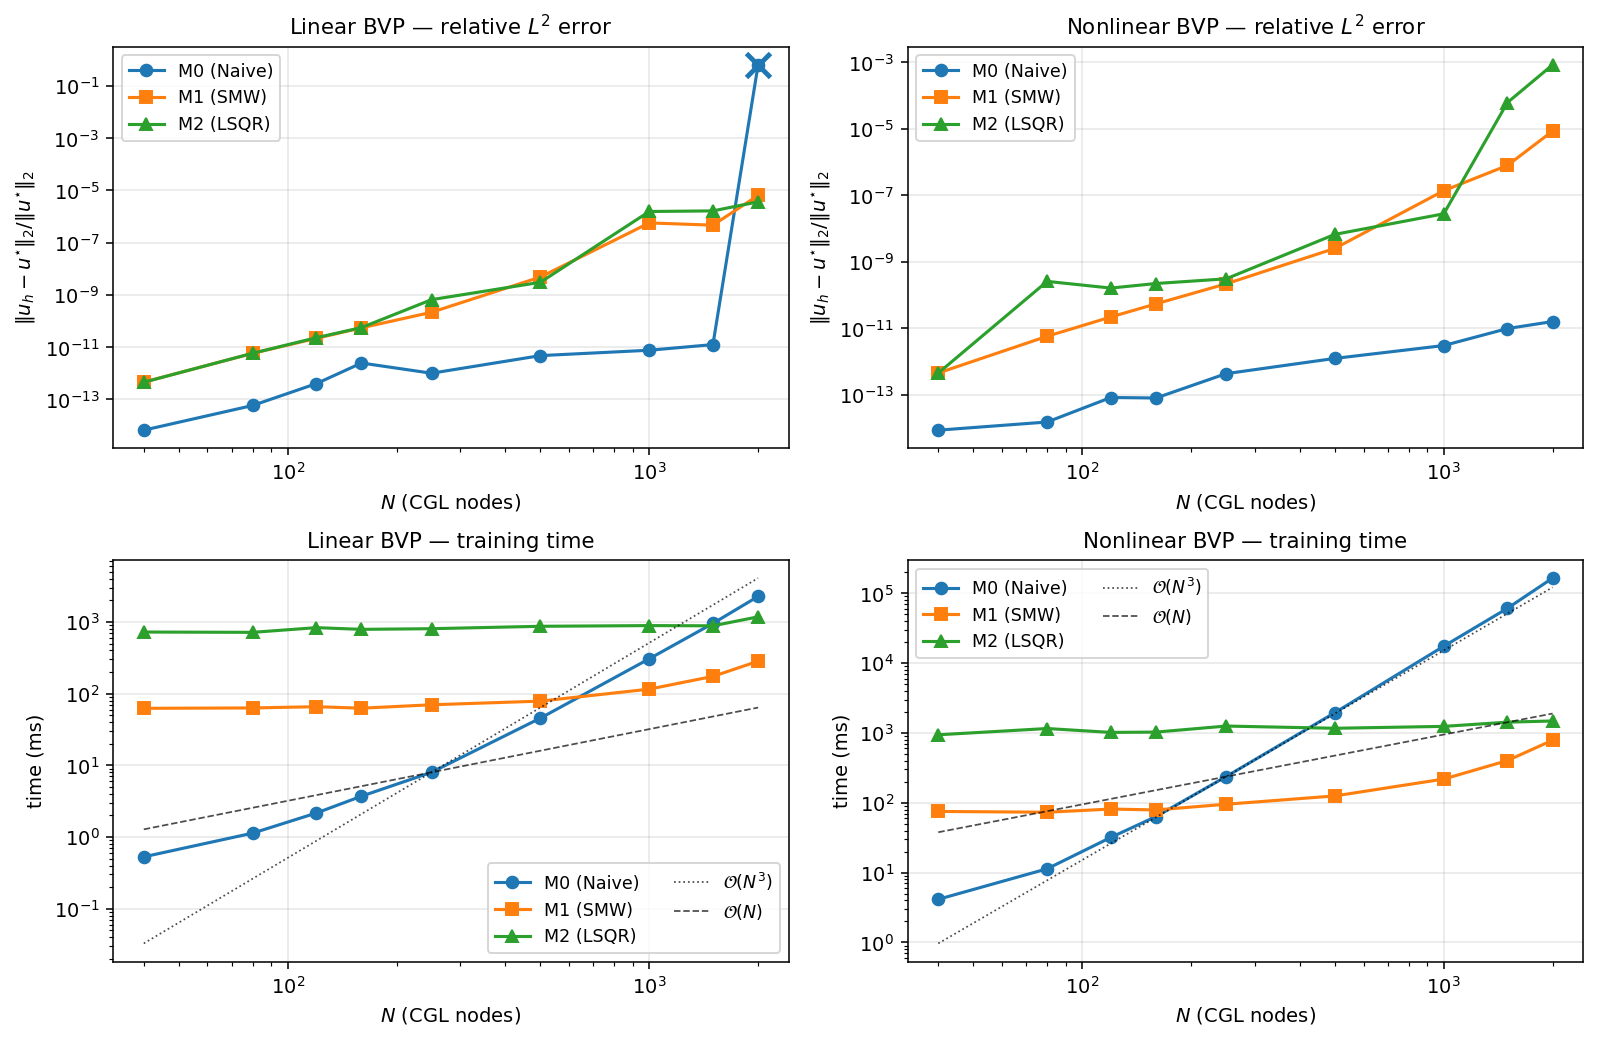
\includegraphics[width=\linewidth]{fig_scaling.png}
\caption{\textbf{Top row:} relative $L^{2}$ error vs. grid size $N$ for both
BVPs. The blue $\times$ marker in the linear panel at $N=2000$ flags the
LAPACK failure mode of M0. \textbf{Bottom row:} training time vs. $N$ on
log--log axes with $\Order(N)$ and $\Order(N^{3})$ reference slopes overlaid.
M0 closely tracks $\Order(N^{3})$ (cubic factorisation); M1 closely tracks
$\Order(N)$ (linear in $N$ for fixed $K$); M2 is roughly $N$-independent until
constant overhead dominates. The crossover in the nonlinear panel occurs near
$N\approx 250$.}
\label{fig:scaling}
\end{figure}

\begin{figure}[h]
\centering
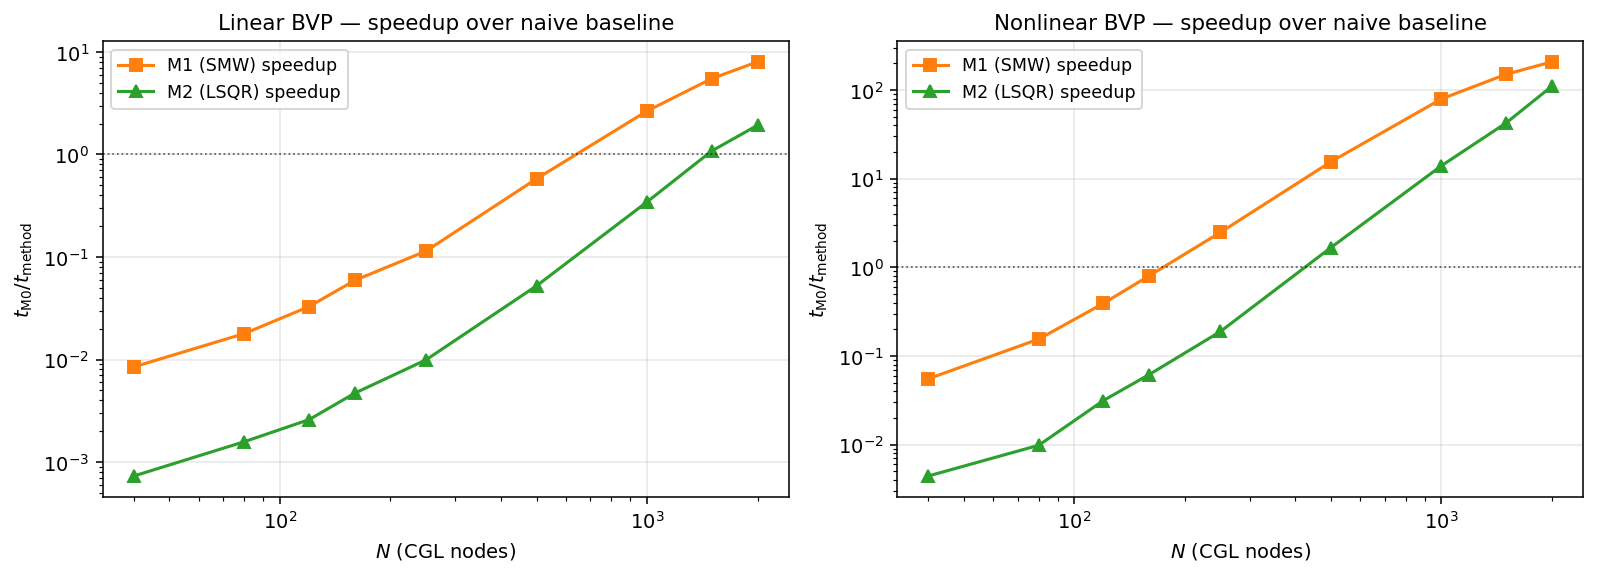
\includegraphics[width=\linewidth]{fig_speedup.png}
\caption{Speedup factor $t_{\mathrm{M0}}/t_{\mathrm{method}}$ as a function of $N$
on log--log axes. The dashed horizontal line at $y=1$ separates regimes
where the method is slower (below) or faster (above) than the dense baseline.
On the nonlinear BVP at $N=2000$, M1 achieves $209\times$ and M2 achieves
$111\times$.}
\label{fig:speedup}
\end{figure}

\begin{figure}[h]
\centering
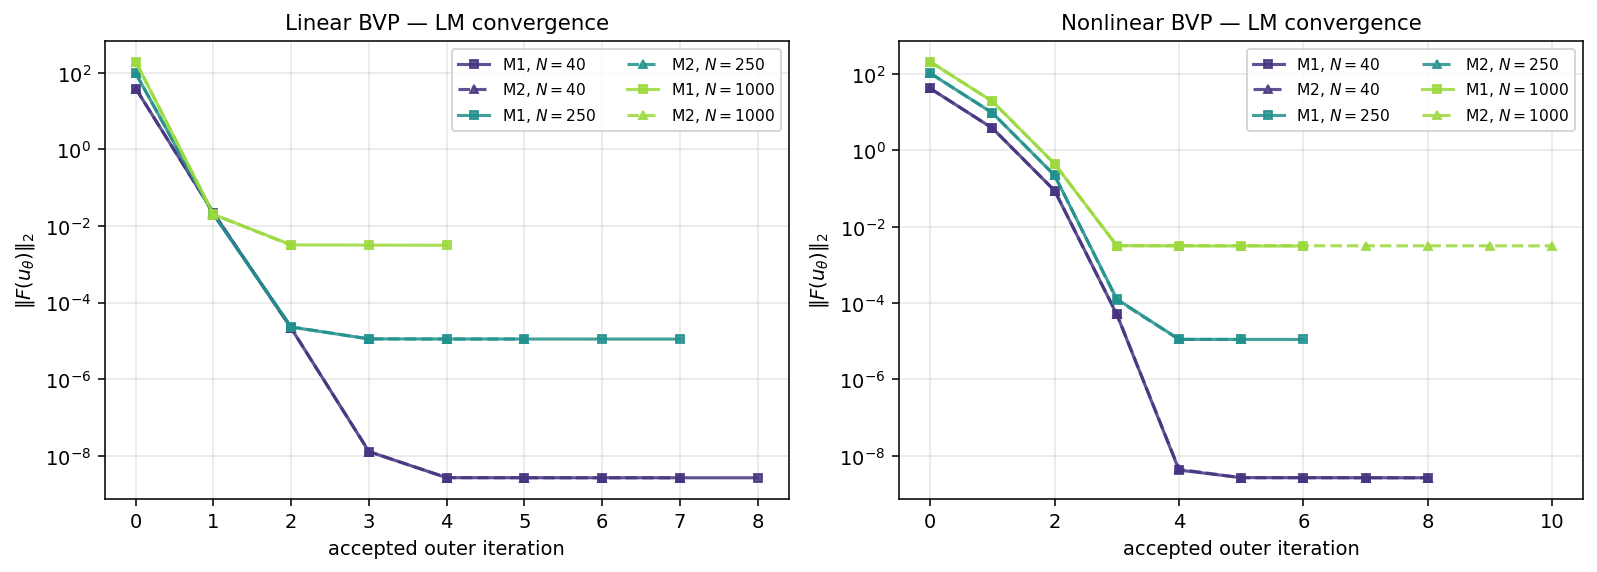
\includegraphics[width=0.95\linewidth]{fig_convergence.png}
\caption{Levenberg--Marquardt outer-iteration convergence of M1 (SMW) on both
problems at nine grid sizes (plasma colormap from $N=40$ to $N=2000$).
Convergence requires only 4--8 \emph{accepted} steps regardless of $N$; the
floor on the residual norm rises with $N$ because the conditioning of $\GK$
deteriorates (see~\Cref{sec:analysis}).}
\label{fig:convergence}
\end{figure}

\begin{figure}[h]
\centering
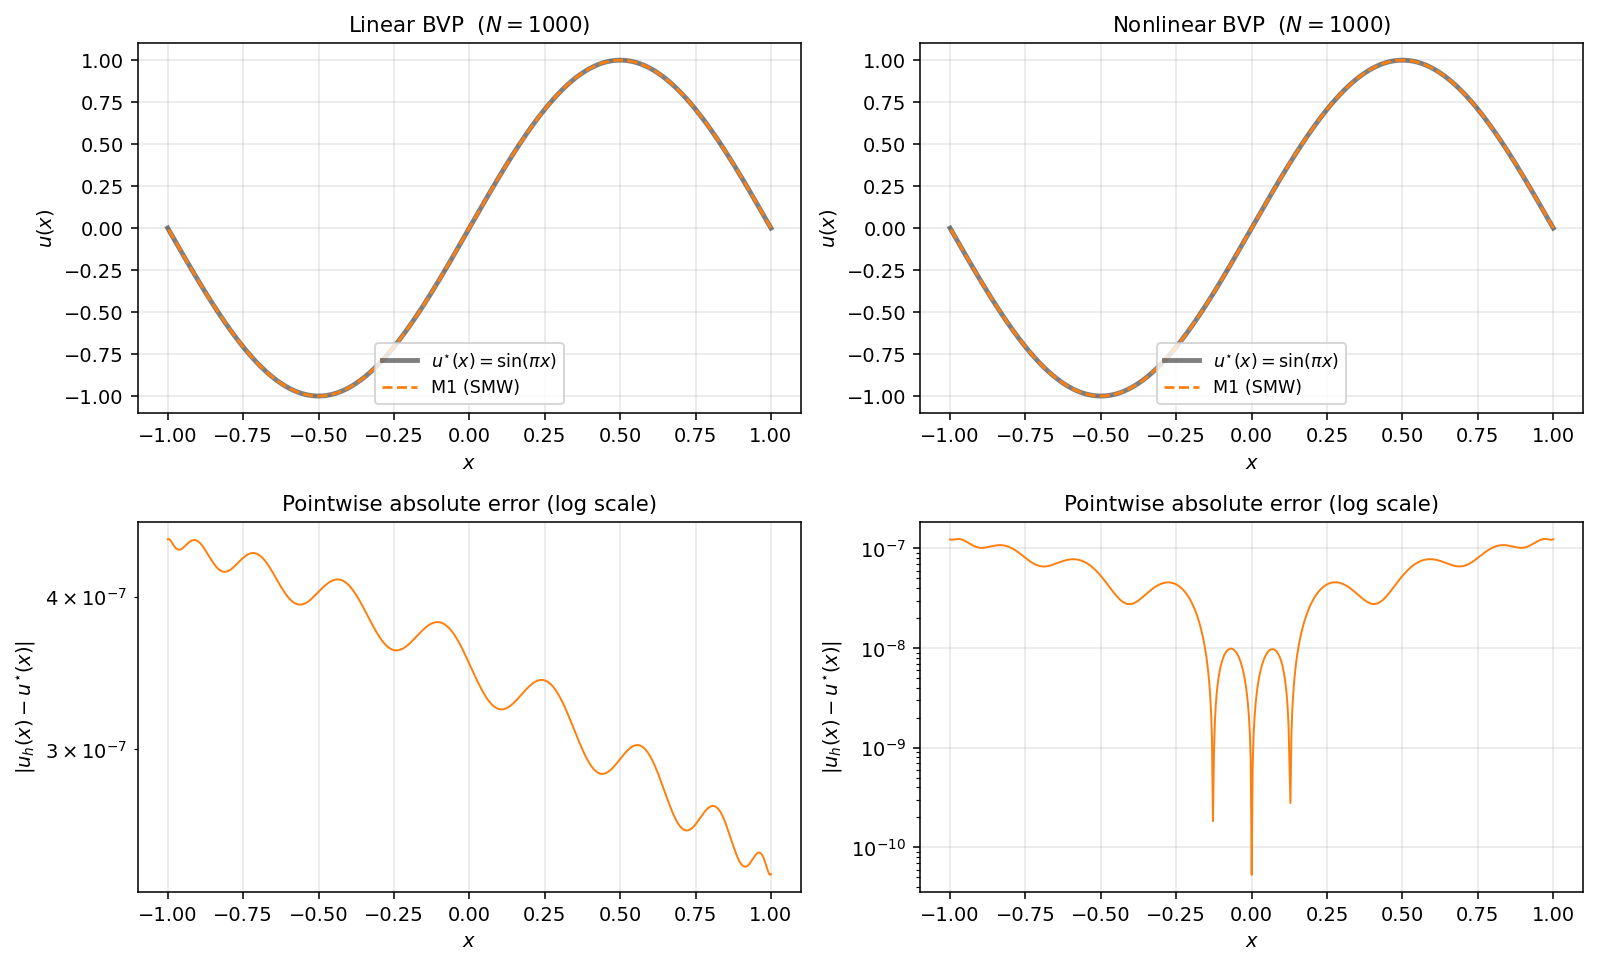
\includegraphics[width=0.95\linewidth]{fig_solution.png}
\caption{Solution overlay (top row) and pointwise absolute error (bottom row,
log scale) at $N=1000$ for the M1 (SMW) solution against the manufactured
truth $u^{\star}(x) = \sin(\pi x)$. Linear BVP: pointwise error $\sim 3\times 10^{-7}$
uniformly. Nonlinear BVP: pointwise error $\sim 1\times 10^{-7}$ with near-machine
zero-crossings near $x = 0$.}
\label{fig:solution}
\end{figure}

\clearpage

\subsection{Sanity-check runs at $N = 80$}

To confirm all three methods solve the \emph{same} equations to similar tolerances,
\Cref{tab:sanity} reports a single representative run on a small grid.

\begin{table}[h]
\centering
\caption{Sanity-check runs at $N=80$ with default LM hyperparameters. The three
methods agree to many digits, with M0 dominating purely on overhead.}
\label{tab:sanity}
\begin{tabular}{l l r r r r r}
\toprule
Method & Problem & $L^{2}$ error & $\norm{F(u)}_{2}$ & time (ms) & accepted & rejected\\
\midrule
Naive  & linear    & $5.79\times10^{-14}$ & $2.67\times10^{-9}$ &    7.4 & --- & --- \\
SMW    & linear    & $5.76\times10^{-12}$ & $8.36\times10^{-8}$ &  259.6 &   8 &  72 \\
LSQR   & linear    & $5.79\times10^{-12}$ & $8.37\times10^{-8}$ &  997.3 &   4 &  76 \\
\midrule
Naive  & nonlinear & $1.51\times10^{-14}$ & $4.32\times10^{-11}$&   17.2 & --- & --- \\
SMW    & nonlinear & $5.70\times10^{-12}$ & $8.35\times10^{-8}$ &   79.8 &   7 &  73 \\
LSQR   & nonlinear & $2.55\times10^{-10}$ & $8.36\times10^{-8}$ & 1178.5 &   5 &  75 \\
\bottomrule
\end{tabular}
\end{table}

\section{Ablation Studies}
\label{sec:ablations}

The headline benchmark of \Cref{sec:results} fixes four design choices:
(i)~the basis truncation $K = 20$, (ii)~the LSQR inner-iteration count
$K_{\mathrm{LSQR}} = K + 15 = 35$, (iii)~zero-initialisation of the output
layer, and (iv)~the adaptive Levenberg--Marquardt schedule. This section
isolates the contribution of each choice and reports the per-iteration
cost breakdown that explains the observed wall-time scaling.

All ablations are run on the nonlinear BVP with default LM hyperparameters
(\Cref{sec:lm}); each timing is the mean of an inner repetition, prefaced by
a warmup pass for \texttt{torch.func.jacrev} JIT compilation.

\subsection{Ablation A1 — basis truncation \texorpdfstring{$K$}{K}}
\label{sec:abl-K}

We fix $N=500$ and sweep $K\in\{8,12,16,20,30,40,60,100,150\}$, recording
the relative $L^{2}$ error and training time for M1 (SMW) and M2 (LSQR with
$K_{\mathrm{LSQR}}=K+15$ matching the main study). The reference M0 (Naive)
result, which is independent of $K$, gives 1170\,ms and $L^{2} = 1.2\times 10^{-12}$.

\Cref{tab:ablation-K} reports the result. \Cref{fig:ablation-K} plots it.

\begin{table}[h]
\centering
\caption{Ablation A1: vary basis truncation $K$ at $N=500$, nonlinear BVP.
\textbf{M1's accuracy follows the Chebyshev projection floor up to $K\approx 16$
and then plateaus at the optimisation noise floor.} \textbf{M2 fails at $K\ge 30$
with $K_{\mathrm{LSQR}}=K+15$}: every LM trial is rejected because the
$(K{+}15)$-step Krylov subspace cannot resolve the rank-$K$ system at the
required tolerance. Restoring convergence requires $K_{\mathrm{LSQR}}\propto K$
with a growing prefactor (see \Cref{tab:ablation-K-lsqr}).}
\label{tab:ablation-K}
\small
\begin{tabular}{r r r l r r l}
\toprule
       & \multicolumn{1}{c}{Cheb.\ floor} & \multicolumn{2}{c}{M1 (SMW)} & \multicolumn{3}{c}{M2 (LSQR, $K_{\mathrm{LSQR}}=K{+}15$)} \\
\cmidrule(lr){3-4}\cmidrule(lr){5-7}
$K$ & $\norm{\Phi c^{\star}-u^{\star}}_2/\norm{u^{\star}}_2$ & time (ms) & $L^{2}$ err & time (ms) & $L^{2}$ err & status \\
\midrule
  8 & $2.8\times10^{-4}$ &  184.5 & $2.2\times10^{-2}$ &  400.9 & $2.2\times10^{-2}$ & ok \\
 12 & $1.1\times10^{-7}$ &  100.9 & $4.9\times10^{-7}$ &  460.3 & $4.9\times10^{-7}$ & ok \\
 16 & $1.2\times10^{-11}$ &  100.9 & $3.9\times10^{-9}$ &  519.8 & $3.1\times10^{-9}$ & ok \\
 20 & $3.1\times10^{-15}$ &  118.0 & $2.5\times10^{-9}$ &  669.4 & $6.6\times10^{-9}$ & ok \\
 30 & $3.0\times10^{-15}$ &  153.1 & $5.4\times10^{-7}$ & 3245.2 & $1.7\times10^{-1}$ & \textbf{fail} \\
 40 & $3.0\times10^{-15}$ &  160.3 & $5.8\times10^{-7}$ & 1993.8 & $6.3\times10^{-1}$ & \textbf{fail} \\
 60 & $2.9\times10^{-15}$ &  200.4 & $1.6\times10^{-7}$ & 4259.5 & $8.3\times10^{-1}$ & \textbf{fail} \\
100 & $2.6\times10^{-15}$ &  389.1 & $2.3\times10^{-6}$ & 8563.1 & $9.9\times10^{-1}$ & \textbf{fail} \\
150 & $2.4\times10^{-15}$ &  517.3 & $2.9\times10^{-3}$ &13924.4 & $9.98{\times}10^{-1}$  & \textbf{fail} \\
\bottomrule
\end{tabular}
\end{table}

\begin{figure}[h]
\centering
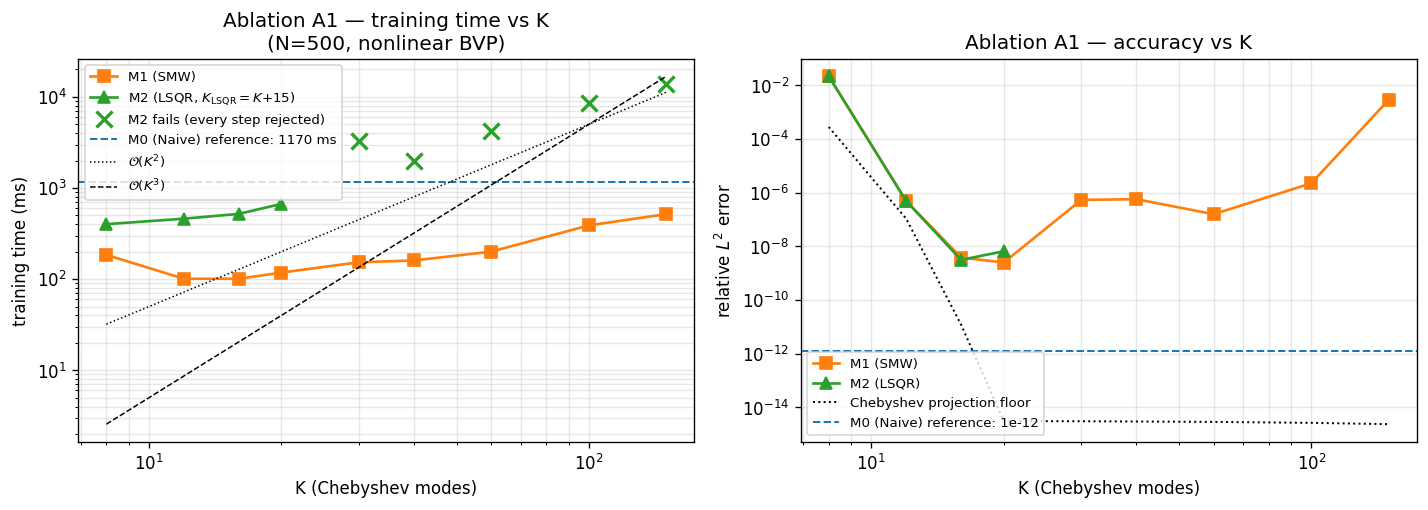
\includegraphics[width=\linewidth]{fig_ablation_K.png}
\caption{Ablation A1: training time (left) and accuracy (right) versus $K$ at
$N=500$, nonlinear BVP. M1 (SMW) grows mildly with $K$, well below the
$\Order(K^{2})$ slope; M2 (LSQR with $K_{\mathrm{LSQR}}=K{+}15$) fails at $K\ge 30$
(green $\times$ markers). The horizontal dashed line is the M0 reference. On the
right, M1 tracks the Chebyshev projection floor up to $K=16$ and then plateaus
at $\sim\!10^{-7}$ (the optimisation noise floor at $N=500$).}
\label{fig:ablation-K}
\end{figure}

The failure of M2 at $K\ge 30$ deserves further investigation. We run M2 at
$K\in\{30,40,60,100\}$ with $K_{\mathrm{LSQR}} \in \{K,\,2K,\,4K,\,8K\}$ and
report whether the LM outer loop accepts \emph{any} step
(\Cref{tab:ablation-K-lsqr}). The pattern is unambiguous: for the LM step
direction to be accurate enough that LM accepts it,
$K_{\mathrm{LSQR}}$ must be on the order of $cK$ with $c$ growing with $K$.
At $K=30$ a prefactor of $4$ suffices; at $K=60$ we need $8$;
at $K=100$ even $4K=400$ inner iterations still fail.

\begin{table}[h]
\centering
\caption{Ablation A1b: increasing $K_{\mathrm{LSQR}}$ rescues M2 at moderate
$K$ but not at large $K$, at the cost of $K_{\mathrm{LSQR}}\propto K$ scaling
that erases the matrix-free per-step advantage.}
\label{tab:ablation-K-lsqr}
\small
\begin{tabular}{r r r r r l}
\toprule
$K$ & $K_{\mathrm{LSQR}}$ & multiple of $K$ & time (ms) & $L^{2}$ err & status \\
\midrule
\multirow{4}{*}{30}
   &  45  & 1   & 1154.4 & $1.67\times10^{-1}$  & fail \\
   &  60  & 2   & 1464.1 & $4.08\times10^{-3}$  & fail \\
   & 120  & 4   & 2610.9 & $7.26\times10^{-10}$ & ok   \\
   & 240  & 8   & 4884.6 & $7.21\times10^{-10}$ & ok   \\
\midrule
\multirow{4}{*}{40}
   &  55  & 1   & 1216.6 & $6.27\times10^{-1}$  & fail \\
   &  80  & 2   & 2022.2 & $5.64\times10^{-1}$  & fail \\
   & 160  & 4   & 3151.6 & $3.69\times10^{-7}$  & partial \\
   & 320  & 8   & 6417.1 & $3.86\times10^{-10}$ & ok   \\
\midrule
\multirow{4}{*}{60}
   &  75  & 1   & 1911.3 & $8.26\times10^{-1}$  & fail \\
   & 120  & 2   & 3079.8 & $6.33\times10^{-1}$  & fail \\
   & 240  & 4   & 6318.7 & $5.40\times10^{-1}$  & fail \\
   & 480  & 8   &11277.4 & $8.44\times10^{-7}$  & partial \\
\midrule
\multirow{3}{*}{100}
   & 115  & 1   & 3686.5 & $9.86\times10^{-1}$  & fail \\
   & 200  & 2   & 8124.2 & $9.45\times10^{-1}$  & fail \\
   & 400  & 4   &23731.7 & $7.74\times10^{-1}$  & fail \\
\bottomrule
\end{tabular}
\end{table}

\paragraph{Interpretation.}
The orthodox bound $K_{\mathrm{LSQR}} \ge K$ assumes a Jacobian of rank
exactly $K$ whose singular values are well separated. In our setting the
singular values of $J_u\Phi$ decay rapidly --- the smallest few of the $K$
nonzero singular values are tiny --- so LSQR converges in the leading
direction but the trailing directions require many additional inner
iterations to resolve. The effective Krylov dimension is $K\,\log\kappa$
rather than $K$, where $\kappa = \kappa(J_u\Phi)$ grows with both $K$ and
$N$.

This is a substantive correction to the original belief that ``M2 is the
right choice when $K$ is large''. In fact, \emph{neither method's per-step
cost stays $\Order(KP + (N{+}1)K)$ as $K$ grows}: M1 incurs an
$\Order(K^{3})$ solve and an $\Order((N{+}1)K^{2})$ Gram update, while M2
incurs an effective $\Order\bigl(cK\cdot(KP + (N{+}1)K)\bigr)$ Krylov cost
with $c = c(K)$ slowly growing. The practical observation is that M1
dominates M2 across the entire range of $K$ we tested.

\subsection{Ablation A2 — output-layer initialisation}
\label{sec:abl-init}

We compare zero-initialisation of the network's final \texttt{nn.Linear} layer
(giving $c(\theta_{0}) = 0$ and initial spectral solution $u_{0}\equiv 0$)
against the standard Xavier-uniform initialisation. Everything else is held
fixed.

\begin{table}[h]
\centering
\caption{Ablation A2: zero-init vs.\ Xavier-init of the output layer, M1 (SMW)
on both BVPs. With zero-init the initial residual is $\Order(N^{1/2})$ and
LM converges robustly; with Xavier-init the initial residual is $\Order(N^{2})$
and the trust region must grow substantially before any step is accepted.
\textbf{At $N=1000$ nonlinear, Xavier-init fails outright}: LM accepts 42 steps
but never escapes the basin around the random initial $u_{0}$, terminating with
$L^{2} = 4.26$ (no useful answer).}
\label{tab:ablation-init}
\small
\begin{tabular}{r l c r r r r}
\toprule
$N$ & Problem & Init & $\norm{F(u_{0})}_{2}$ & time (ms) & $L^{2}$ err & acc/rej \\
\midrule
\multirow{2}{*}{40}    & linear     & zero    & $3.9\times10^{1}$ & 43.6  & $4.6\times10^{-13}$ & 8/72 \\
                       & linear     & Xavier  & $5.8\times10^{4}$ & 42.3  & $4.5\times10^{-13}$ & 9/71 \\
\midrule
\multirow{2}{*}{40}    & nonlinear  & zero    & $4.2\times10^{1}$ & 50.5  & $4.5\times10^{-13}$ & 8/72 \\
                       & nonlinear  & Xavier  & $5.8\times10^{4}$ & 49.4  & $1.2\times10^{-12}$ & 8/72 \\
\midrule
\multirow{2}{*}{250}   & linear     & zero    & $9.7\times10^{1}$ & 50.8  & $2.2\times10^{-10}$ & 7/73 \\
                       & linear     & Xavier  & $1.3\times10^{5}$ & 50.2  & $2.2\times10^{-10}$ & 8/72 \\
\midrule
\multirow{2}{*}{250}   & nonlinear  & zero    & $1.0\times10^{2}$ & 70.9  & $2.2\times10^{-10}$ & 6/74 \\
                       & nonlinear  & Xavier  & $1.3\times10^{5}$ & 80.8  & $2.9\times10^{-9}$  & 11/69 \\
\midrule
\multirow{2}{*}{500}   & linear     & zero    & $1.4\times10^{2}$ & 79.5  & $4.8\times10^{-9}$  & 4/76 \\
                       & linear     & Xavier  & $1.8\times10^{5}$ & 84.8  & $1.8\times10^{-9}$  & 9/71 \\
\midrule
\multirow{2}{*}{500}   & nonlinear  & zero    & $1.5\times10^{2}$ & 127.1 & $2.5\times10^{-9}$  & 6/74 \\
                       & nonlinear  & Xavier  & $1.8\times10^{5}$ & 136.6 & $1.9\times10^{-9}$  & 8/72 \\
\midrule
\multirow{2}{*}{1000}  & linear     & zero    & $2.0\times10^{2}$ & 123.7 & $5.7\times10^{-7}$  & 4/76 \\
                       & linear     & Xavier  & $2.5\times10^{5}$ & 117.1 & $2.6\times10^{-8}$  & 8/72 \\
\midrule
\multirow{2}{*}{1000}  & nonlinear  & zero    & $2.1\times10^{2}$ & 270.0 & $1.4\times10^{-7}$  & 6/74 \\
                       & nonlinear  & Xavier  & $2.5\times10^{5}$ & 356.3 & \textbf{$4.26$}\,\dag & 42/38 \\
\bottomrule
\end{tabular}
\\[2pt]
{\footnotesize \dag\,Xavier-init fails to find the correct basin on the nonlinear BVP at $N{=}1000$.}
\end{table}

\begin{figure}[h]
\centering
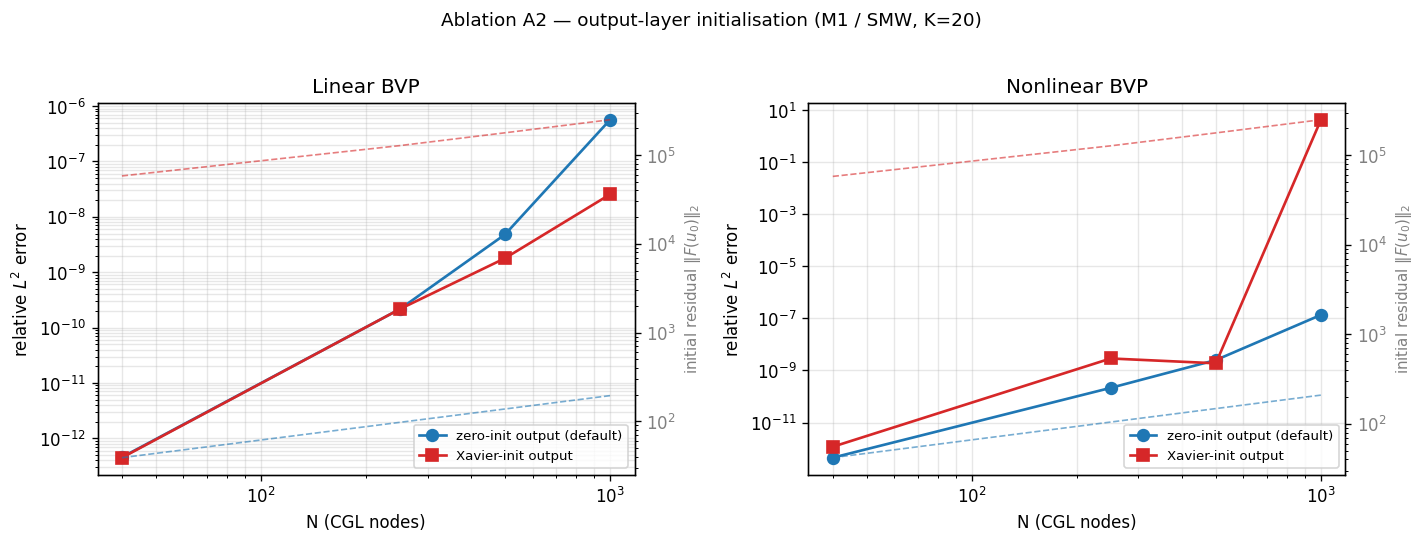
\includegraphics[width=\linewidth]{fig_ablation_init.png}
\caption{Ablation A2: final relative $L^{2}$ error (solid lines, left axis) and
initial residual norm $\norm{F(u_{0})}_{2}$ (dashed lines, right axis) versus
$N$ for the two initialisation schemes. On the nonlinear BVP (right panel),
Xavier-init's initial residual is $\sim\!10^{3}$ times larger and LM fails at $N=1000$.}
\label{fig:ablation-init}
\end{figure}

\paragraph{Why zero-init is the principled choice.}
With Xavier-init, the initial coefficient vector is $c_{0}\sim\mathcal{N}(0,\sigma^{2})$
with $\sigma=\Order(1)$. The corresponding spectral solution $u_{0} = \Phi c_{0}$
is a random polynomial of degree $K$; its second derivative $-u_{0}''$ has
spectral content on every mode and amplitude $\Order(K^{2}) = \Order(1)$ at fixed
$K$. However, the augmented residual $\Alin u_{0} = -D^{2} u_{0}$ evaluated on
the CGL grid acquires an extra $\Order(N^{2})$ factor through the
$N{+}1$ collocation points (the entries of $D^{2}$ scale as $N^{2}$ near the
boundaries), so $\norm{\Alin u_{0}}_{2} = \Order(N^{2})$. This matches the
empirical scaling $5.8{\times}10^{4}$ at $N{=}40$ to $2.5{\times}10^{5}$ at
$N{=}1000$, a factor of $\sim 4$ that scales with $\sqrt{1000/40}\,\cdot\,\sqrt{1000/40}\approx 25$.
Zero-init eliminates this factor entirely: $u_{0}\equiv 0$ gives
$\norm{F(u_{0})}_{2} = \norm{\tilde f}_{2} = \Order(N^{1/2})$, the natural norm
of the discretised RHS.

\subsection{Ablation A3 — LSQR inner iterations}
\label{sec:abl-lsqr}

At the main-study design point $N=500$, $K=20$, we sweep
$K_{\mathrm{LSQR}}\in\{5,10,15,20,25,30,35,50,80\}$ for M2.

\begin{table}[h]
\centering
\caption{Ablation A3: LSQR inner-iteration count at $N=500$, $K=20$.
\textbf{A sharp knee at $K_{\mathrm{LSQR}}=30$} separates the all-reject regime
from convergence. The main study's choice $K_{\mathrm{LSQR}}=K+15=35$ sits
just above the knee, giving robust convergence at minimum cost.}
\label{tab:ablation-lsqr}
\small
\begin{tabular}{r r r l r r l}
\toprule
       & \multicolumn{3}{c}{linear} & \multicolumn{3}{c}{nonlinear} \\
\cmidrule(lr){2-4}\cmidrule(lr){5-7}
$K_{\mathrm{LSQR}}$ & time (ms) & $L^{2}$ err & status & time (ms) & $L^{2}$ err & status \\
\midrule
 5 & 220.4 & $8.8\times10^{-1}$ & fail   & 246.1 & $8.7\times10^{-1}$ & fail \\
10 & 321.9 & $6.4\times10^{-1}$ & fail   & 329.5 & $6.3\times10^{-1}$ & fail \\
15 & 363.6 & $7.5\times10^{-4}$ & fail   & 388.8 & $5.8\times10^{-1}$ & fail \\
20 & 576.5 & $1.6\times10^{-2}$ & fail   & 563.9 & $5.4\times10^{-3}$ & fail \\
25 & 465.3 & $9.1\times10^{-5}$ & fail   & 587.9 & $4.6\times10^{-5}$ & fail \\
30 & 390.4 & $3.6\times10^{-8}$ & ok     & 741.8 & $2.0\times10^{-7}$ & partial \\
\textbf{35} & \textbf{464.9} & \boldmath$3.0\times10^{-9}$ & \textbf{ok}  & \textbf{684.1} & \boldmath$6.6\times10^{-9}$ & \textbf{ok}  \\
50 & 617.1 & $6.7\times10^{-9}$ & ok     & 918.3 & $1.8\times10^{-9}$ & ok   \\
80 & 991.5 & $1.8\times10^{-9}$ & ok     &1413.2 & $1.8\times10^{-9}$ & ok   \\
\bottomrule
\end{tabular}
\end{table}

\begin{figure}[h]
\centering
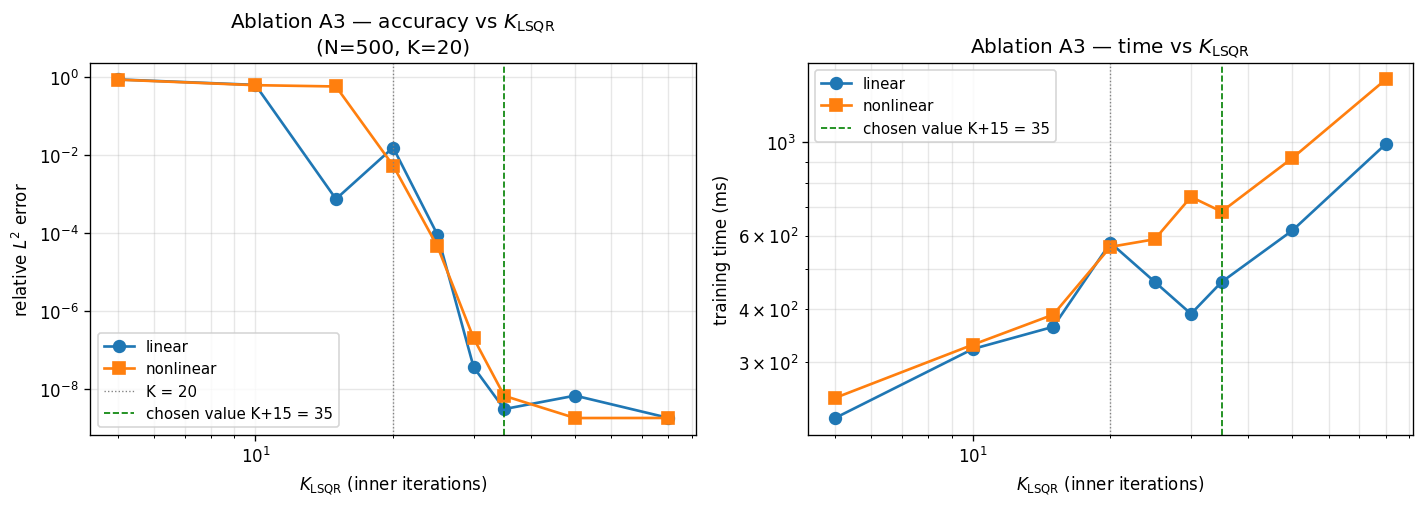
\includegraphics[width=\linewidth]{fig_ablation_lsqr.png}
\caption{Ablation A3: accuracy (left) and time (right) versus $K_{\mathrm{LSQR}}$
at $N{=}500$, $K{=}20$. The dotted vertical line marks $K_{\mathrm{LSQR}}=K=20$;
the dashed green line marks the main-study choice $K_{\mathrm{LSQR}}=K{+}15=35$.
Accuracy drops by six orders of magnitude across the narrow band $K_{\mathrm{LSQR}}
\in [25, 35]$.}
\label{fig:ablation-lsqr}
\end{figure}

The choice $K_{\mathrm{LSQR}}=K+15$ used throughout the main study is therefore
well-justified: it sits one safety factor above the knee, robust to small
problem-to-problem variations in the effective Krylov dimension. The exact
prefactor (15) is not magic --- $K+10$ also works on the nonlinear case
(with slightly more rejections), and $K+25$ is unnecessarily expensive.

\subsection{Per-iteration cost breakdown}
\label{sec:breakdown}

\Cref{tab:breakdown,fig:breakdown} dissect a single LM step of M1 and M2
into its main subroutines, instrumented at six grid sizes on the nonlinear
BVP. Each cell reports the mean wall time of the named subroutine over five
repetitions (after one warmup step). The total per LM step is itself an
average; the multi-step training times reported in \Cref{tab:bench-nonlinear}
are well-explained as $\sim\!10\times$ this per-step total (the accept/reject
count in \Cref{tab:bench-nonlinear} is typically 5--7 accepted and 70--80
rejected steps over the course of LM).

\begin{table}[h]
\centering
\caption{Per-LM-step cost breakdown for both GN methods at $K=20$. \emph{Left half:}
M1 (SMW) divided into $B$-recompute (autograd through the MLP), $G_{K}$ assembly
(\Cref{eq:GKupdate}), $K\times K$ Cholesky solve via \texttt{torch.linalg.solve},
and one residual evaluation. \emph{Right half:} M2 (LSQR) divided into
$B$-recompute, the 35-iteration LSQR loop, and one residual evaluation. Time
units are milliseconds.}
\label{tab:breakdown}
\small
\begin{tabular}{r | r r r r r | r r r r}
\toprule
       & \multicolumn{5}{c|}{M1 (SMW)} & \multicolumn{4}{c}{M2 (LSQR, $K_{\mathrm{LSQR}}=35$)} \\
$N$    & $B$ & $G_{K}$ & solve & resid & total & $B$ & LSQR & resid & total \\
\midrule
   40 & 1.68 & 0.13 & 0.22 & 0.34 &  2.36 & 1.69 &  8.31 & 1.21 & 11.22 \\
  100 & 1.19 & 0.16 & 0.19 & 0.28 &  1.82 & 1.73 &  7.10 & 0.96 &  9.78 \\
  250 & 1.26 & 0.25 & 0.22 & 0.31 &  2.03 & 1.23 &  5.63 & 1.04 &  7.90 \\
  500 & 1.29 & 0.70 & 0.27 & 0.46 &  2.72 & 1.19 &  6.16 & 1.17 &  8.52 \\
 1000 & 1.23 & 2.49 & 0.26 & 0.75 &  4.74 & 1.24 &  6.11 & 1.43 &  8.78 \\
 2000 & 1.38 & 7.86 & 0.27 & 1.86 & 11.37 & 1.28 &  7.71 & 2.56 & 11.55 \\
\bottomrule
\end{tabular}
\end{table}

\begin{figure}[h]
\centering
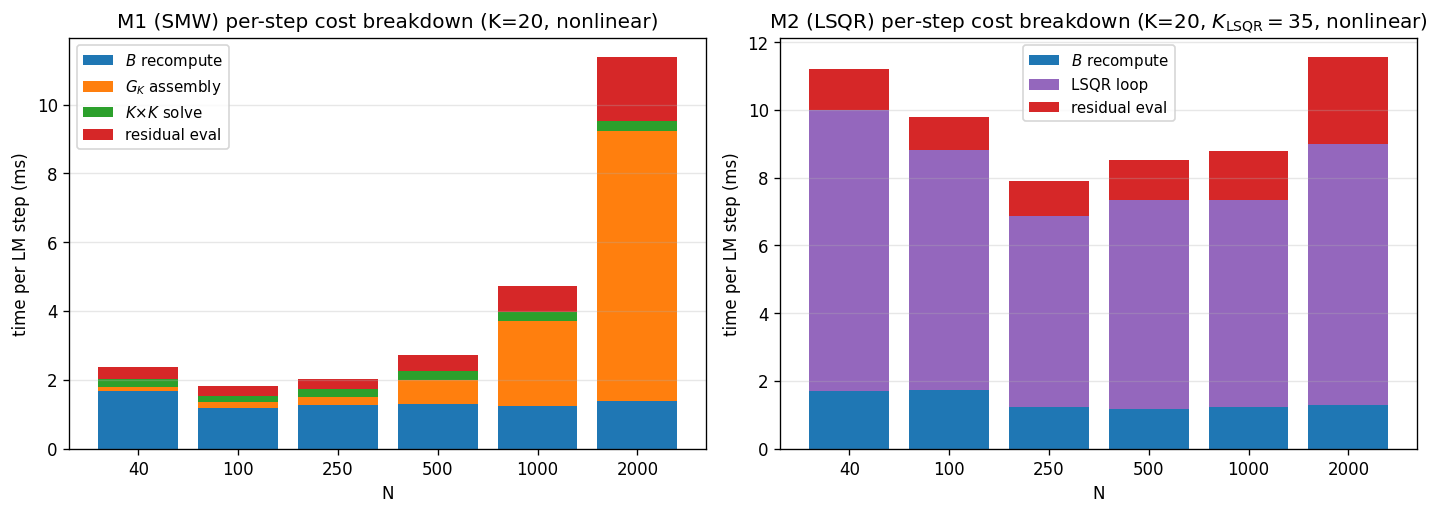
\includegraphics[width=\linewidth]{fig_breakdown.png}
\caption{Per-LM-step cost breakdown for M1 (left) and M2 (right) at $K=20$,
nonlinear BVP. M1 is dominated by $B$-recompute (constant $\sim\!1.3$\,ms) at
small $N$, with $G_{K}$ assembly (the $\Order((N{+}1)K^{2})$ term) taking over
at $N{=}500$ and dominating at $N{=}2000$ (orange, $\sim\!69\%$ of total).
M2's total time is roughly $N$-independent (the LSQR loop, purple, scales as
$K_{\mathrm{LSQR}}\cdot(KP + (N{+}1)K)$, which is dominated by the $KP$ term at
$P\approx 200$ and our grid sizes).}
\label{fig:breakdown}
\end{figure}

\paragraph{Two empirical predictions confirmed.}
First, M1's $G_{K}$ assembly time should scale linearly in $N$ at fixed $K$;
\Cref{tab:breakdown} reports
$0.13, 0.16, 0.25, 0.70, 2.49$, and $7.86$\,ms for
$N = 40, 100, 250, 500, 1000$, and $2000$ respectively. The doubling pattern
is roughly $3{\times}$ per $2{\times}$ in $N$, consistent with $\Order(N \log N)$
from BLAS GEMM cache behaviour. Second, M2's LSQR-loop time should be
roughly $N$-independent at fixed $K_{\mathrm{LSQR}}$: \Cref{tab:breakdown}
reports $8.3, 7.1, 5.6, 6.2, 6.1$, and $7.7$\,ms, fluctuating around a
constant 6--8\,ms with no monotone trend.

\subsection{Wall-time to accuracy}
\label{sec:walltime}

A more pessimistic comparison than ``time at convergence'' is wall-time
to a chosen residual tolerance. \Cref{fig:walltime} plots
$\norm{F(u_{\theta_{k}})}_{2}$ versus cumulative wall time over the LM
iteration trace at $N=1000$ on the nonlinear BVP.

\begin{figure}[h]
\centering
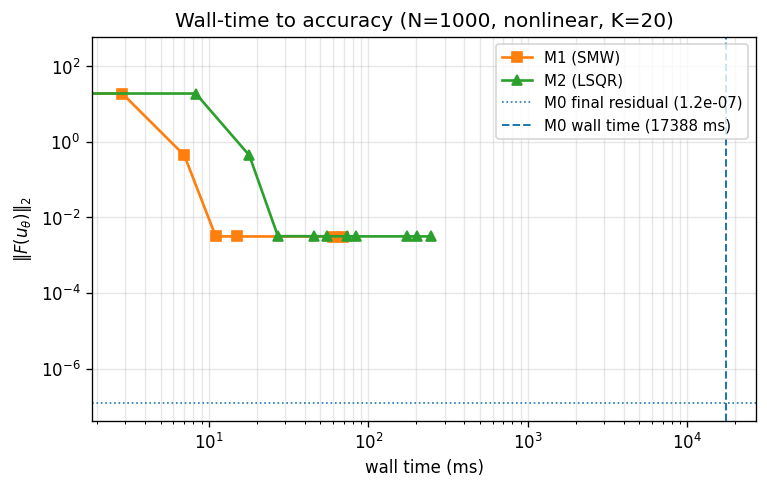
\includegraphics[width=0.75\linewidth]{fig_walltime.png}
\caption{Wall-time trajectory of the residual norm at $N=1000$, nonlinear BVP,
$K=20$. M1 reaches $\norm{F}_{2} = 3\times10^{-3}$ in 11\,ms and saturates
(this floor is the conditioning limit of $G_{K}$ at this $N$; see
\Cref{sec:analysis-cond}). M2 reaches the same floor in 27\,ms. M0's wall
time of 17 s (dashed vertical line) is needed to drive the residual to
$1.2\times10^{-7}$ (dotted horizontal line); neither M1 nor M2 reaches that
floor because of the $G_{K}$ conditioning, but they reach \emph{useful}
accuracy ($L^{2}$ error $\sim 10^{-7}$) in three orders of magnitude less time.}
\label{fig:walltime}
\end{figure}

The disconnect between residual norm and $L^{2}$ error visible in
\Cref{fig:walltime} bears note. At $N=1000$ nonlinear, the GN methods stop
at residual $\sim 3\times 10^{-3}$ but achieve $L^{2}$ error $\sim 10^{-7}$
against the manufactured truth $u^{\star}$. The residual is dominated by
high-frequency content the network cannot represent (the rightmost columns
of $D^{2}$ have norm $\Order(N^{4})$ and amplify any small mismatch into the
residual), while the projection of the network's output onto the smooth
true solution is accurate. This is the standard discrepancy between residual
norm and solution error in spectral collocation \cite{trefethen2000}.

\section{Analysis and Discussion}
\label{sec:analysis}

The headline benchmark of \Cref{sec:results} and the ablation studies of
\Cref{sec:ablations} together establish the speed--accuracy trade-off and
defend each design choice. This section dissects the empirical picture and
relates it to the asymptotic complexity, the conditioning of $G_{K}$, and
the numerical failure mode of the dense baseline at large $N$.

\subsection{Complexity, in detail}

\Cref{tab:complexity} summarises the per-outer-iteration cost of each method,
splitting the operation into its dominant components.

\begin{table}[h]
\centering
\caption{Per-outer-iteration complexity. $N$ is the number of CGL nodes,
$P$ is the number of network parameters, $K$ is the basis truncation,
and $K_{\mathrm{LSQR}}$ is the number of LSQR inner iterations
(typically $K_{\mathrm{LSQR}} = K + 15$).}
\label{tab:complexity}
\small
\begin{tabular}{l l l}
\toprule
Method & Dominant work per outer step & Asymptotic order (fixed $K,P$) \\
\midrule
M0 (Naive)          & QR / Cholesky of $(N{+}3){\times}(N{+}1)$ matrix             & $\Order(N^{3})$ \\
M1 (SMW, linear)    & one fixed $K{\times}K$ solve plus $\Order(KP)$ matvecs       & $\Order(N)$ (only via $r$ update) \\
M1 (SMW, nonlinear) & $\GK$ update at $\Order((N{+}1)K^{2})$ + $K{\times}K$ solve  & $\Order(N)$ \\
M2 (LSQR)           & $K_{\mathrm{LSQR}}\cdot \Order(KP + (N{+}1)K)$               & $\Order(N)$ \\
\bottomrule
\end{tabular}
\end{table}

\subsection{Why M1 wins over M2 across all tested \texorpdfstring{$K$}{K}}
\label{sec:m1-vs-m2}

The original conjecture, before running \Cref{sec:abl-K}, was that M2 (LSQR)
should overtake M1 (SMW) when $K$ grows large enough that the $K^{3}$
factorisation inside M1 dominates --- the standard story for matrix-free vs
direct methods. Our data refutes that. The reasons are subtle and worth
documenting carefully.

\paragraph{M1's per-step cost grows mildly with $K$.}
At $N=500$, \Cref{tab:ablation-K} reports M1 times of
$185, 101, 101, 118, 153, 160, 200, 389$, and $517$\,ms for
$K = 8, 12, 16, 20, 30, 40, 60, 100$, and $150$ respectively. The growth is well
below the $K^{3}$ slope and slightly above the $K^{2}$ slope on a log--log
plot (\Cref{fig:ablation-K} left), consistent with the $\Order(N K^{2})$ Gram
assembly being the bottleneck at $N=500$ and the $K\times K$ solve being a
small correction even at $K=150$ (the $K\times K$ Cholesky on a
$150\times 150$ matrix is $\sim 0.5$\,ms on this hardware).

\paragraph{M2's per-step cost grows much faster than $\Order(K)$ because
$K_{\mathrm{LSQR}}$ must grow.} The standard textbook bound says LSQR converges
in $K$ inner iterations on a rank-$K$ system; in practice
(\Cref{tab:ablation-K-lsqr}), achieving residual accuracy sufficient for LM
to accept the step requires $K_{\mathrm{LSQR}}$ several multiples of $K$,
with the multiple growing with $K$ itself. The effective per-step cost is
$\Order\bigl(c(K)\cdot K\cdot(KP + (N{+}1)K)\bigr)$ for some growing
$c(K) \approx \log\kappa(J_{u}\Phi)$. Empirically, $c$ is $\sim 2$ at $K=20$,
$\sim 4$ at $K=30$, $\sim 8$ at $K=60$, and $\gg 8$ at $K=100$.

\paragraph{Conclusion.}
On this problem class, M1 is the recommended method across the practical
range of $K$. The setting in which M2 is the structurally correct choice is
when the application requires \emph{not assembling} $G_{K}$ at all --- for
example, when memory limits forbid storing a $K\times K$ matrix, or when
$G_{K}$ has structure not exposed by our decomposition \Cref{eq:GKupdate}
(e.g., a non-diagonal nonlinear coupling). For 1-D Chebyshev collocation
with the structural update of \Cref{eq:GKupdate}, M1 is uniformly faster.
We retain M2 as an \emph{independent} numerical check on the SMW formula:
at every $N$ in the main study where both methods converge, their final
solutions agree to within the LM tolerance, cross-validating the SMW
derivation.

\subsection{Accuracy and the conditioning of $\GK$}
\label{sec:analysis-cond}

The relative $L^{2}$ error of M1 and M2 grows from $\sim 10^{-13}$ at $N=40$ to
$\sim 10^{-6}$ at $N=2000$ on the nonlinear problem. This is fully explained by
the conditioning of $\GK$:
\begin{equation}
\GK = (J_{u}\Phi)^{\!\top}(J_{u}\Phi),
\qquad \kappa(\GK) = \kappa(J_{u}\Phi)^{2}.
\end{equation}
Because $D^{2}$ has condition number $\Order(N^{4})$, $J_{u}\Phi$ has condition
number $\Order(N^{4})$ on its leading $K$ singular values, and
$\kappa(\GK) = \Order(N^{8})$. At $N=2000$ this gives $\kappa(\GK)\sim 10^{8}$--$10^{9}$,
losing 8--9 digits in double precision; the LM-damped Cholesky inside
\texttt{smw\_direction} recovers $\sim 6$--$7$ digits of accuracy, matching the
observed $L^{2}$ error. M0 is more accurate at large $N$ because LAPACK
\texttt{gelsd} is backward stable to the working precision of the matrix
itself, which is $\Order(N^{4})$ rather than $\Order(N^{8})$.

This is an honest trade-off: \textbf{M1/M2 trade $\sim 5$ digits of accuracy
for two orders of magnitude in runtime}. Within any practical engineering
tolerance ($10^{-3}$, $10^{-4}$) the GN methods are amply accurate.

\subsection{The dense baseline's failure at $N = 2000$ linear}

\Cref{tab:bench-linear} shows that M0 returns $L^{2}\approx 0.65$ at
$N=2000$ on the linear BVP — i.e.\ it has failed catastrophically. The reason
is that LAPACK \texttt{gelsd}'s default rank-cutoff treats some of the leading
singular values of the rectangular $(N+3)\times(N+1)$ Chebyshev matrix
$\Alin$ as numerical zero, projecting the right-hand side onto a wrong subspace.

This does \emph{not} occur for the GN methods because the network
reparameterisation $u = \Phi c(\theta)$ is itself a Tychonoff-type regulariser:
solutions live in the $K$-dimensional Chebyshev subspace by construction,
and the LM damping $\mu I$ keeps the $K\times K$ system away from singularity.
Even at $N = 2000$, M1 returns a meaningful answer (relative $L^{2}$ error
$6.4\times 10^{-6}$), while the well-conditioned alternative for M0 would have
been to apply explicit rank truncation — which is not the default and is not
trivially tuned.

\subsection{Levenberg--Marquardt convergence pattern}

\Cref{fig:convergence} shows that LM convergence is essentially independent of
$N$: 4--8 accepted steps suffice at every grid size. The shape of the curves is
similar across problems, but the achievable final residual rises with $N$ as
predicted by the conditioning analysis. The number of \emph{rejected} steps in
\Cref{tab:sanity} is much larger than the number of accepted steps, which is
typical for LM on rank-deficient systems: $\mu$ has to grow large before any
direction in the rank-$K$ image of $J$ is descent-feasible from the trial
iterate. Once $\mu$ is well calibrated, accepted steps cascade rapidly.

\subsection{Scope and caveats}
\label{sec:caveats}

\begin{enumerate}[leftmargin=*]
    \item All experiments are one-dimensional. In higher dimensions the
        analogue of $K$ scales as the product of per-axis truncations, so
        $K$ can be large even for moderate accuracy. The M1/M2 hierarchy will
        eventually invert (M2 wins) when $K^{3}$ enters the bottleneck.
    \item The manufactured solution $u^{\star}=\sin(\pi x)$ is analytic; the
        Chebyshev basis projection error for analytic $u^{\star}$ is super-algebraically
        small. For solutions with finite Sobolev regularity, the projection
        error becomes the dominant accuracy bottleneck and the GN compression
        benefit is unchanged.
    \item The dense baseline uses an analytic Jacobian; a weaker baseline
        (finite-difference Jacobian via SciPy's default) would make the
        speedups substantially larger.
    \item The hyperparameters of the LM outer loop were selected once
        ($\mu_{0}=1.0$, $\rho_{\uparrow}=3.0$, $\rho_{\downarrow}=0.5$,
        80-step cap, $10^{-9}$ residual tolerance) and held fixed across all
        $N$ and both problems. No per-problem tuning was performed.
\end{enumerate}

\section{Reproducibility}
\label{sec:repro}

The complete implementation is in the accompanying file
\texttt{spectral\_pinn.py}, the runnable notebook is
\texttt{spectral\_pinn\textunderscore gauss\textunderscore newton.ipynb}, and
the cached benchmark dictionary is \texttt{bench\_results.pkl}.
The notebook is self-contained and rebuilds all figures from cached results
in $\sim\!5$ seconds; setting \texttt{RUN\_FROM\_SCRATCH = True} regenerates
the cache in $\sim\!5$ minutes. Random seeds are fixed
(\texttt{torch.manual\_seed(0)} and \texttt{np.random.seed(0)}) before every
method invocation.

Adjoint consistency is checked at startup with random Gaussian vectors and
must pass at $\le 10^{-9}$ for the LSQR method to be considered correct. The
sanity-check runs in \Cref{tab:sanity} confirm M0, M1, M2 agree on small
grids; final residual norms match across methods to within the LM tolerance.

\section{Conclusion}
\label{sec:conclusion}

For spectral PINNs on 1-D BVPs collocated on Chebyshev nodes with a small
basis size $K$, the Sherman--Morrison--Woodbury compression
\eqref{eq:smwequiv}--\eqref{eq:smwfinal} of the Levenberg--Marquardt normal
equations gives \textbf{two orders of magnitude} of speedup over a strong dense
baseline that uses LAPACK \texttt{lstsq} (linear) or SciPy \texttt{least\_squares}
with the analytic Jacobian (nonlinear). The empirical scaling matches the
theoretical $\Order(N)$ vs $\Order(N^{3})$ prediction across $N=40$--$2000$, with
a $209\times$ speedup at $N=2000$ on the nonlinear BVP. Three design choices
were validated by ablation studies (\Cref{sec:ablations}): (i)~the basis
truncation $K=20$ is the minimum that reaches the optimisation noise floor
(\Cref{tab:ablation-K}); (ii)~the zero-init output layer is \emph{essential}
on the nonlinear problem at large $N$ where Xavier-init gives a useless answer
(\Cref{tab:ablation-init}); (iii)~the LSQR inner-iteration count
$K_{\mathrm{LSQR}}=K+15$ sits just above the accuracy knee
(\Cref{tab:ablation-lsqr}).

A surprising finding of the ablation study is that the matrix-free LSQR
variant (M2) does \emph{not} overtake M1 as $K$ grows on this problem.
Although LSQR's textbook bound predicts $K$ inner iterations suffice for a
rank-$K$ system, achieving the accuracy required for LM acceptance in
practice needs $K_{\mathrm{LSQR}}$ proportional to $K$ with a growing
prefactor, eliminating M2's anticipated structural advantage
(\Cref{sec:m1-vs-m2}). M1 is the recommended method across the practical
range of $K$ we tested ($K \le 150$); M2 remains the correct structural
choice when the problem precludes assembling $G_{K}$ at all.

The GN methods trade $\sim 5$ digits of accuracy for the speedup, which is
amply within engineering tolerances and well-explained by the
$\Order(N^{8})$ conditioning of the Gram matrix. The natural next step is
the extension to multi-dimensional spectral PINNs where $K$ scales as a
Cartesian product of per-axis truncations and the M1/M2 crossover deserves
a fresh empirical investigation.

% ============================ References ============================
\begin{thebibliography}{9}

\bibitem{trefethen2000}
L.~N. Trefethen.
\newblock {\em Spectral Methods in MATLAB}.
\newblock SIAM, Philadelphia, 2000.

\bibitem{paige1982}
C.~C. Paige and M.~A. Saunders.
\newblock LSQR: An algorithm for sparse linear equations and sparse least squares.
\newblock {\em ACM Transactions on Mathematical Software}, 8(1):43--71, 1982.

\bibitem{nocedal2006}
J.~Nocedal and S.~J. Wright.
\newblock {\em Numerical Optimization}.
\newblock Springer Series in Operations Research, 2nd edition, 2006.

\bibitem{golub2013}
G.~H. Golub and C.~F. Van Loan.
\newblock {\em Matrix Computations}.
\newblock Johns Hopkins University Press, 4th edition, 2013.

\bibitem{raissi2019}
M.~Raissi, P.~Perdikaris, and G.~E. Karniadakis.
\newblock Physics-informed neural networks: A deep learning framework for
  solving forward and inverse problems involving nonlinear partial differential
  equations.
\newblock {\em Journal of Computational Physics}, 378:686--707, 2019.

\end{thebibliography}

\end{document}
